\def\bibliocommand{\bibliography{bibliography}}
\input{latBegin.txt}

\chapter{Abstract}
\label{abstract}

The importance of fungi in the ecosystem cannot be overestimated. Not only are they key decomposers, they also provide food and digestive aid to many animals, and most plants rely on fungi living in their roots for minerals, nutrients and protection. This relationship between plants and fungi is what is known as a mycorrhizal symbiosis. One group of plants, the Orchidaceae, are particularly reliant on this symbiosis, as their seeds do not contain nutritional resources and are obligately dependent on a fungal symbiont to provide nutrients in order to germinate and reach phosynthetic stage. Despite this importance, the ecological processes that influence the distribution of fungi, and the associated environmental and biotic factors, are still unclear.

Fungi are often invisible to human eye and the soil is a very complex system, containing many organisms. By sampling the specific obligate fungi that live in the orchid roots, orchid mycorrhizal funghi (OrM) we can explore the ecological mechanisms that contribute to their distribution.

In this study I constructed a database of all known European OrM and used a combination of phylogenetic analysis, multivariate analysis and hierarchical species distribution modelling. I found that OrM families were phylogenetically distinct, but that OTUs were poorly resolved. Multivariate analysis revealed that precipitation and soil chemical variables (mainly potassium) were important in determining the distribution of OrM. Hierarchical species distribution modelling revealed that most OrM taxa had either positive or negative residual cooccurrence, indicating that ecological mechanisms such as competition and facilitation may be important to explain the distribution of OrM. The results presented here represent a useful starting point for detailed experiments for understanding important belowground interactions and conservation of soil biodiversity.

\textbf{Keywords:} \emph{fungal ecology, mycorrhizas, orchidaceae, hierarchical model of species community, joint species distribution model}

\chapter{Riassunto}
\label{riassunto}

L'importanza dei funghi negli ecosistemi non può essere sovrastimata. Oltre ad essere decompositori chiave, forniscono cibo e supporto digestivo a molti animali, mentre la maggior parte delle piante dipende dai funghi che vivono nelle loro radici per minerali, nutrienti e protezione. Questa relazione tra piante è funghi è nota come simbiosi micorrizica e un gruppo di piante, le Orchidaceae, sono particolarmente dipendenti da questa simbiosi. I loro semi non contengono nutrienti e dipendono dai funghi per ottenere i nutrienti necessari alla germinazione e al raggiungimento dello stadio fotosintentico. Nonostante ciò, i processi ecologici che influenzano la distribuzione dei funghi, e i fattori ambientali e biotici associati, sono ancora poco chiari.

I funghi sono solitamente invisibili all'occhio umano e il suolo è un sistema molto complesso, in cui vivono molti organismi. Campionando i funghi che vivono nel sistema radicale delle orchidee, i funghi micorrizici delle orchidee (FMO), possiamo esplorare i meccanismi ecologici che contribuiscono alla loro distribuzione.

In questo studio ho costruito un database di tutti i funghi micorrizici conosciuti in Europa e ho usato una combinazione di analisi filogenetica, analisi multivariata e modellistica gerarchica di distribuzione delle specie. Ho trovato che le famiglie di FMO sono filogeneticamente distinte, ma a livello delle unità tassonomiche operative (OTU) i risultati non sono ben risolti. L'analisi multivariata ha rivelato che le precipitazioni e le caratteristiche chimiche del suolo (principalmente il potassio) sono importanti nel determinare la distribuzione dei FMO. La modellistica gerarchica di distribuzione delle specie ha rivelato che la maggior parte dei taxa di FMO hanno una correlazione nella presenza, positiva o negativa, a indicazione che meccanismi ecologici come competizione e facilitazione potrebbero essere importanti per spiegare la distribuzione dei FMO. I risultati presentati rappresentano un utile punto di partenza per futuri esperimenti e per comprendere importanti interazioni nel suolo e la conservazione della biodiversità.

\textbf{Parole chiave:} \emph{ecologia dei funghi, micorrize, orchidaceae, hierarchical model of species community, joint species distribution model}

\part{Introduction}
\label{introduction}

The kingdom Fungi is one of the most diverse groups of organisms on Earth. Fungi play an important role in the ecosystem and have a huge impact on biogeochemical cycles, plant and animal pathology, plant nutrition and soil properties.
While historically fungi were taxonomically clustered with plants ~\citep{copeland1938, copeland1956}, towards the middle of the twentieth century it became clear that it failed to properly deal with the differences between the two groups. In 1969 R. H. Whittaker divided organisms into five kingdoms: Animalia, Plantae, Fungi, Protista and Monera ~\citep{whittaker1969}. By the 1970s this division became widely accepted, and the Kingdom Fungi was recognized.
However, due to a limited understanding of the taxonomy, evolution and phylogenesis of fungi, it was still a matter of ample debate. All the analysis were based on morphological differences, which limited our understanding of what represents a species in this group.

The fossil record for fungi is limited and even though the known fossils cover almost all major fungal lineages ~\citep{lucking2009}, it is rather incomplete relative to the evolutionary history of the various fungal lineages. The earliest compendium of fossil fungi is from the late 19th century ~\citep{meschinelli1898}, and their symbiotic relationship with plants in fossils was suggested around that period ~\citep{renault1896}, but the difficulty in the interpretation of morphological data made it impossible to actually understand what happened.

The earliest fossil with the morphological features of a fungus is dated to around 1 billion years ago, and was found in the Canadian Arctica ~\citep{loron2019}, and there is evidence of fungus-like organisms in fossils of around 800 Mya ~\citep{bonneville2020}.
Starting from the lower Devonian (around 400 Mya), fossil record is more abundant ~\citep{lucking2009}.

It was not until the development of molecular phylogenetics techniques that some light could be properly shed on the evolutionary history of fungi ~\citep{james2006}.

The molecular clock is one of the most widely used tools to investigate the timing of phylogenetic events. It is based on the hypothesis of the constancy of the rate of evolution with time and, when combined with the use of fossil records, allows the dating of branching events on phylogenetic trees ~\citep{lepage2007, weir2008}.
From molecular clock analysis seems like fungi are sister group to animals, that is, the two lineages are close, diverging around 1.5 billion years ago ~\citep{wang1999}. The two groups form one supergroup called Opisthokhonta ~\citep{cavalier-smith1987}, from the Greek opísthios (rear, posterior) and kontós (``pole'' i.e. ``flagellum''), since the group is characterized by flagellate cells that propel themselves with a single, posterior flagellum, now lost in most fungi ~\citep{steenkamp2006} with the notable exception of the Chytridiomycota division ~\citep{james2006a}.

\begin{figure}[htbp]
\centering
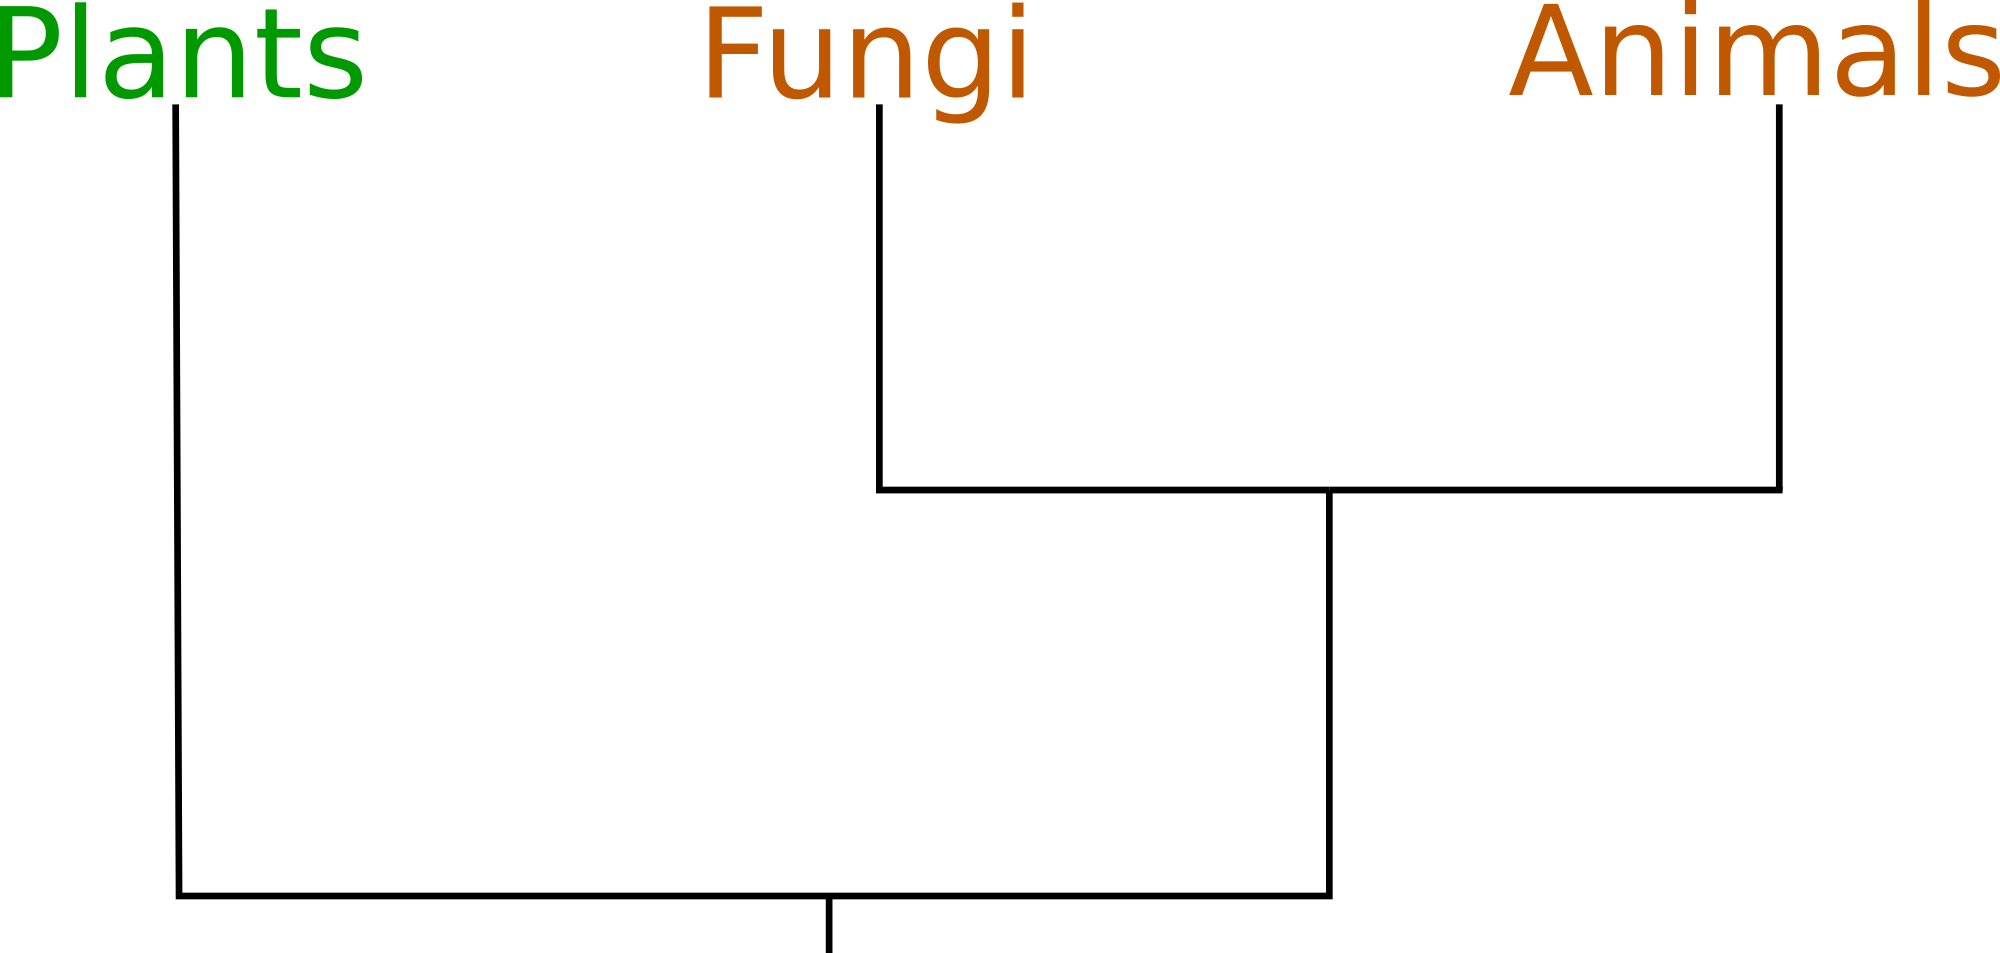
\includegraphics[keepaspectratio,width=\textwidth,height=0.75\textheight]{images/pfatree.png}
\caption{Simplified phylogenetic tree showing the relationship between the three clades}
\end{figure}

The ancestors of fungi are believed to be simple aquatic forms with flagellated spores, similar to members of the extant phylum Chytridiomycota (chytrids), which are now considered one of the early-diverging clade in the kingdom ~\citep{james2006}. The first terrestrial fungi colonized land probably before plants ~\citep{heckman2001}, as saprobe (taking nutrition out of dead matter) and\slash or in symbiosis with organisms capable of photosynthesis.
It is commonly accepted that in order to colonize the land, plants had to develop a symbiotic relationship with fungi ~\citep{selosse1998, heckman2001, bonneville2020}, but it is not entirely clear whether this relationship was lichen-like (an algae or cyanobacteria living among filaments of a single or more fungi) ~\citep{spribille2016} or mycorrhizal-like, where the fungus colonizes the host plant's root tissues.

Lichens are the symbiotic relationship between a single or more fungi (\emph{mycobiont}) and a cyanobacteria or algae (\emph{photobiont}). Early plants that transitioned from aqueous environments were poorly equipped to deal with the challenges of a terrestrial life style: mainly, to decompose the mineral substrate to absorb nutrients, to protect itself against dehydration, UV radiations and temperature fluctuations ~\citep{selosse1998, blackwell2000}. By forming relationships with fungi (i.e. a lichen), the photobiont is protected by the fungal stroma, and it can tolerate drought, cold, heat, intense light and barren rocky substrates. Indeed they also seem to be pioneers of harsh environments today.

Yet, while the relationship between plants and fungi evolved several times ~\citep{gargas1995}, the only fungal group we know that are capable of forming such association (called \emph{lichenization}) are Ascomycota and Basidiomycota. The origin of those clades can be dated to about 400 Mya in the Devonian period ~\citep{berbee1993}. Similarly there are fossils for lichens dating at the oldest in the Early Devonian (400 Mya) ~\citep{taylor1997, honegger2013}, while the first fossil land plants and fungi appeared 480 to 460 Mya, and molecular clock estimates suggests about 600--700 Mya ~\citep{berbee1993, heckman2001}.

Therefore, lichens were likely not what opened the way to plants for land colonization.

The mycorrhizal association is a symbiotic association between plants and fungi happening in the rhizosphere, the plant's root system ~\citep{barman2016}. In this interaction there is an exchange of resources between the mycorrhizal fungus and the plant, ideally the plant providing sugar to the fungus and the fungus providing minerals and nutrients to the plant. However, this is not always the case and upon closer analysis, there appears to be a continuum of plant responses to mycorrhizal colonization ranging from positive to neutral to negative, and the same goes for the fungi ~\citep{johnson1997}.

Fossils resembling mycorrhizal relationships date to the Ordovician (with an age of about 460 million years), and are Glomales-like Arbuscular Mycorrhizal Fungi (AMF hereafter), in a moment where the land flora was comprised mainly of bryophytes, pteridophytes and algae ~\citep{redecker2000}. Plants can photosynthetize; these fungi can extract minerals from the substrate with great efficiency, protect the root system, extend the range from which water can be taken and protect the plants from pathogens.

Fossil records provides evidence that fungal organisms entered in such symbiosis before the appearance of true roots, and as long as there is a multicellular host AM fungi are fine ~\citep{wang2006, bonfante2008}.

Whether as lichen or as mycorrhiza, the symbiosis between plants and fungi is one of the most important, most ancient relationship in the history of living beings and it surely played a crucial role in the successful colonization of the land by plants ~\citep{pirozynski1975, malloch1980, harley1987, trappe1987, selosse1998, brundrett2002}. The relationship is so beneficial (for one or both parts) that today is the norm, and is well established in c. 85\% of extant plants ~\citep{cairney2000, strullu-derrien2018}, with a high degree of complexity ~\citep{heijden2015} and mycorrhizal networks often constitute 20\%–30\% of total soil microbial biomass ~\citep{leake2011}

\chapter{Orchid-mycorrhizal fungi relationship}
\label{orchid-mycorrhizalfungirelationship}

Orchidaceae is a diverse and widespread family of flowering plants, containing over 28,000 species in about 736 genera ~\citep{christenhusz2016}, second only to Asteraceae in terms of species numbers ~\citep{ramirez2007}. They are cosmopolitan, with a distribution spanning all continents except Antarctica and including most major island groups ~\citep{givnish2016}.
By the end of 2017 the IUCN Global Red List included assessments for 948 orchid species, of which 56.5\% are threatened ~\citep{fay2018}. In Europe all wild orchids are protected, being included in their entirety on Appendices I and II of the Convention on International Trade in Endangered Species of Wild Fauna and Flora ~\citep{CITES-1} as are many of the habitats they live in, and are listed on the Red List of many countries. Nonetheless, this protection has not staved off a general decline in the orchid flora of Europe ~\citep{jacquemyn2005, kull2006}. Major threats include habitat destruction and unsustainable (often illegal) harvesting, and because of their complex life histories orchids are thought to be particularly vulnerable to the effects of global environmental change ~\citep{kull2016, gale2018}.

Orchids exhibit a high diversity of habitat adaptations, morphologies and pollination strategies, but some characteristics are common to the whole family. One of the most important is the reliance on Orchid Mycorrhizal Fungi (OrM here after) for reproduction and survival. This is because orchids seeds are devoid of nutritional resources, and they completely rely on fungi for nutrition including water, minerals and carbon supply ~\citep{leake1994, rasmussen1998, merckx2013} in a nutritional strategy called ``mycoheterotrophy''. After germination, seedlings often become autotrophic and subsequently revert to usual mycorrhizal functioning ~\citep{rasmussen1995, cameron2008}. Some species, especially from forest environments, remain mycoheterotrophic at adulthood though, developing partial photosynthetic capacity but still relying on fungi for carbon resources, a nutritional strategy called ``mixotrophy'' or ``partial mycoheterotrophy'' ~\citep{gebauer2003, julou2005, selosse2009}. Others never develop photosynthetic capacity and therefore rely completely on fungi for nutrition. This nutritional mode, which has evolved over 30 times independently in orchids, is called ``obligate mycoheterootrophy'' ~\citep{merckx2013}.

While the relationship between orchids and OrM is known for over a century ~\citep{bernard1899, rayner1927, rasmussen2002, selosse2011} and the mechanisms of this symbiosis are beginning to be properly understood, the knowledge from a taxonomical standpoint is still unclear. For many years orchids were thought to interact almost entirely with a specific clade of fungi, members of the Rhizoctonia complex. It was later discovered not only that orchids have way more interactions with different fungi also from the Ascomycetes phylum, but also that Rhizoctonia is a polyphyletic group, and was disassembled in different taxa, all members of the Agaricomycetes, most notably Sebacinales, Ceratobasidiaceae and Tulasnellaceae ~\citep{dearnaley2012}.
There is also evidence of fungi from the Ascomycota phylum, especially in the order Pezizales ~\citep{selosse2004, ouanphanivanh2008, waterman2011}, but they are the exception: the most common and known families of OrM are in the Basidiomycota phylum, particularly Inocybaceae, Tulasnellaceae, Ceratobasidiaceae, Russulaceae, Sebacinaceae, Serendipitaceae and Thelephoraceae ~\citep{taylor2004, roy2009, duffy2019}

\section{Distribution and ecology of orchid mycorrhizal fungi}
\label{distributionandecologyoforchidmycorrhizalfungi}

Orchids depend on OrM for the germination of their seeds and in many cases for nutrient provision also in adulthood, we assume that OrM must co-occur with the orchid population. However, many OrM can also turn to a soil free-living saprotrophic ecological niche ~\citep{oberwinkler2017} and form mycorrhizal relationships with plants other than orchids ~\citep{selosse2014}. Members of the Tulasnellaceae, Ceratobasidiaceae, and Sebacinales (Serendipitaceae and Sebacinaceae) are ubiquitous, with varying relative abundances ~\citep{jacquemyn2017}.

Environmental factors that underlie the distribution of OrM taxa are poorly understood. Abiotic variables such as annual rainfall, temperature regimes and soil chemical properties should explain the distribution of many taxa. However, local biotic interaction, community composition and interactions may influence the OrM distribution, especially considering they are symbiotic organisms ~\citep{jacquemyn2017}. Overall, there is a lack of evidence, and many parts of the world are undersampled (e.g. all the African continent and most of the tropical areas of the planet). Therefore, it is difficult to conclude that the occurrence of OrM taxa are structured by biotic variables based on a limited amount of data. A part of the problem is that the relationships between orchids and OrM are complex. They both vary in their degree of specialization, from a highly specialized to a more generalist ~\citep{mccormick2004, girlanda2011, heijden2015}, and OrM may be able to revert to saprophytic free-living lifestyles~\citep{veldre2013}.

In this thesis, I investigate the distribution and ecological factors underlying the occurrence OrM throughout Europe. I analyzed the OrM taxa associated with 16 different orchid species that occur in different regions throughout Europe. Specifically, I focus on two over-arching questions:

\begin{enumerate}
\item do similar OrM taxa occur in similar habitats and have similar environmental preferences?

\item Are similarities in OrM co-occurrence explained better by positive environmental correlations or are there residual taxa correlations that may suggest ecological processes beyond environmental filtering (e.g. competition and facilitation)?

\end{enumerate}

\part{Materials and methods}
\label{materialsandmethods}

Data regarding the distribution of OrM in Europe were entered into a database. The data included were composed of OrM fungi isolated from orchid roots, and were georeferenced to the nearest known locality; also, each sample had to have a Genbank accession code in order to obtain the sequences and do the analysis.
Only sequences from well-known OrM were considered, that is: Ceratobasidiaceae, Inocybaceae, Russulaceae, Sebacinaceae, Serendipitaceae, Thelephoraceae and Tulasnellaceae ~\citep{dearnaley2012}.
Orchid species sampled were \emph{Cephalanthera damasonium} ~\citep{julou2005}, \emph{Cephalanthera longifolia} ~\citep{pecoraro2017}, \emph{Dactylorhiza baltica} ~\citep{shefferson2008}, \emph{Epipactis atrorubens} ~\citep{shefferson2008}, \emph{Himantoglossum adriaticum} ~\citep{pecoraro2013}, \emph{Limodorum abortivum} ~\citep{girlanda2005}, \emph{Neottia cordata} ~\citep{tesitelova2015}, \emph{Neottia ovata} ~\citep{hansjacquemyn2015, tesitelova2015}, \emph{Ophrys bertolonii} ~\citep{pecoraro2015}, \emph{Orchis anthropophora}~\citep{julou2005}, \emph{Orchis militaris} ~\citep{shefferson2008}, \emph{Orchis purpurea} ~\citep{lievens2010}, \emph{Orchis simia} ~\citep{schatz2010, lievens2010}, \emph{Orchis tridentata} ~\citep{pecoraro2012}, \emph{Spiranthes spiralis} ~\citep{duffy2019}.

For each georeferenced population six variables were extracted by using the ESDAC database ~\citep{panagos2012} and the WorldClim database ~\citep{hijmans2005}: Nitrogen, Potassium and Phosphorus soil content, soil pH, minimum temperature of the coldest quarter and maximum precipitation of the wettest month. These variables were selected because mycorrhizal fungi may be sensitive to nutrients in the soil: Nitrogen, Phosphorus and Potassium in high quantities (such as in eutrophicated soils because of agricultural fertilizers) have been seen to cause decline in the belowground mycorrhizal fungi species richness and cause dramatic changes in the community composition and structure ~\citep{lilleskov2002, baar2002, grant2011}. Mycorrhizal fungi growth and community composition also seem to be influenced by the soil pH ~\citep{aarle2002, carrino-kyker2016}, temperature and precipitation ~\citep{rillig2003}. Those variables may serve as important proxy for other conditions. Biomes and vegetation are correlated with the environmental conditions, because they change local conditions (like soil pH). Also, human impact can often be seen by the amount of chemicals in the soil, especially close to cultivated fields.
Environmental values were extracted using \texttt{GDAL}'s \texttt{Sample Raster Values} tool (Using QGIS v. 3.16 as a GUI) and appended to the dataset

\begin{figure}[htbp]
\centering
\includegraphics[keepaspectratio,width=\textwidth,height=0.75\textheight]{images/map.png}
\caption{\textbf{Geographical distribution of sampling locations of members from OrM families used in this study} (Basemap Imagery ©2021 TerraMetrics, Map data ©2021 GeoBasis-DE\slash BKG (©2009), Google, Inst Geogr. Nacional)}
\end{figure}

\chapter{Phylogenetic analysis}
\label{phylogeneticanalysis}

In order to understand the distribution and ecology of the OrM we need a better insight of their phylogenesis. The hypothesis was for sequences of the same family to be clustered together, with some doubts regarding the Sebacinales as Serendipitaceae and Sebacinaceae are very closely related and have only been recently separated ~\citep{weiss2016}.
Phylogenetic analysis were performed on the sequences deposited by the papers included in the database.
The primers used were mainly ITS1F, ITS4, ITS3 and ITS4OF, all targeting regions between the 18S rRNA subunit and the 28S rRNA subunit, including the Internal Transcribed Spacers (ITS hereafter) 1 and ITS 2. Those primers were usually universal for Basidiomycota or in some cases more specific for Tulasnellaceae (like ITS4tul) or other taxa.
Sequence \texttt{DQ520100} from \emph{Tremiscus helvelloides} was used as outgroup.

\begin{itemize}
\item Sequences were aligned using the MUSCLE algorithm ~\citep{edgar2004} and manually trimmed to a visually satisfying overlapping;

\item Ugene was used as main GUI, v. 37.0 ~\citep{okonechnikov2012};

\item Maximum Parsimony analysis was performed using TNT, v. 1.1 ~\citep{tnt}, using the Tree Bisection and Reconnection algorhithm and with ten replics. 1000 trees were kept and a strict consensus tree was calculated. Bootstrap analysis was performed on the tree with 200 replications to test the validity of the tree. Bootstrap values are displayed as node labels in the appendix tree (Appendix 1);

\item the Bayesian analysis (MCMC) was performed using MrBayes, v. 3.2.7a ~\citep{huelsenbeck2001}, using the Hasegawa-Kishino-Yano with a gamma rate heterogeneity among sites (\texttt{lset nst=2 rates=gamma;}). One million trees were generated and sampled each thousand, with four chains running. A final consensus tree was then calculated (see appendix).

\item Trees were then visually edited with FigTree v. 1.4.4.

\item All parameters are available in the supplemental data, along with the files to reproduce the analysis.

\end{itemize}

\chapter{Multivariate analysis}
\label{multivariateanalysis}

Before proceeding with the multivariate analysis, sequences have been clustered into Operative Taxonomic Units (OTU hereafter), by using cd-hit v. 4.8.1 ~\citep{li2001}. This process yielded 210 OTUs, with the extremes of Serendipitaceae having two OTUs only, and Tulasnellaceae 52 OTUs.
The database was then pivoted in a presence-absence matrix, and for further analysis it was splitted by family, so that each matrix only had all the OTUs for that single family, yielding seven different matrices. This was necessary to test what variability each family has; another matrix was obtained by grouping together all the observations from the same family, to test the variability between the different OrM families.

\begin{figure}[htbp]
\centering
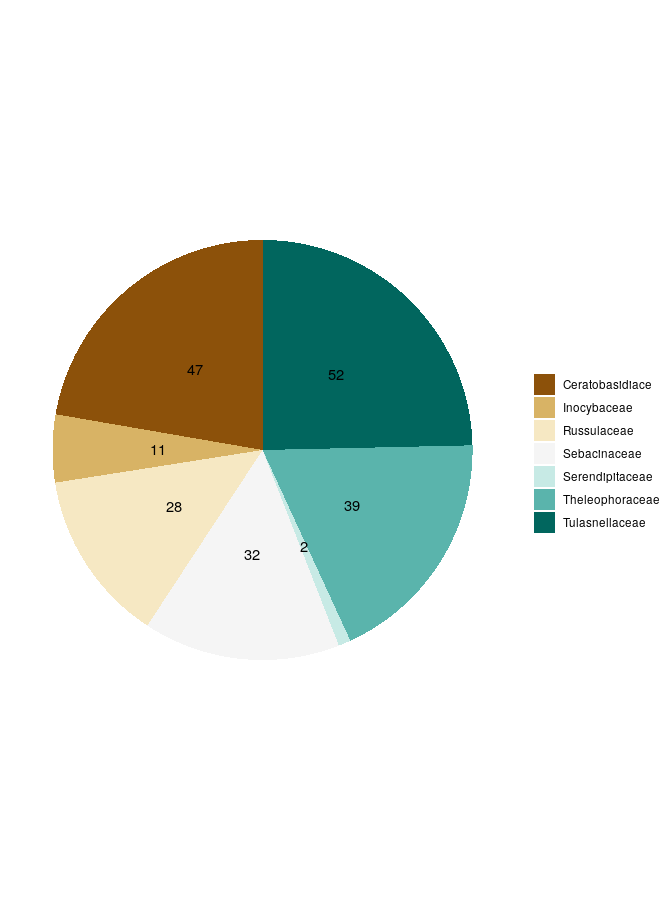
\includegraphics[keepaspectratio,width=\textwidth,height=0.75\textheight]{images/clust.png}
\caption{Number of OTUs from each OrM family}
\end{figure}

A final matrix was obtained by using the single families\slash OTUs as rows and removing orchid species as a variable. This was done to understand the impact of the environmental variables only on each OTU, therefore trying to understand how different the realized niche (i.e. the variance in the environmental variables) is between the groups.

Principal Component Analysis (PCA hereafter) is an orthogonal linear transformation of the data that aims to maximize the variance of the scalar projection of all points of a dataset into a number of axis ordinated by explained variance. This yields a set of axis, which can be used for clustering, to reduce the number of dimensions and perform other analysis. PCA was performed on all matrices using the base R functions \texttt{princomp()}, which takes into account the covariance matrix and applies an eigen method of spectral decomposition when possible. Only in the case of Russulaceae, when the number of observation was too limited, \texttt{prcomp()} was used, which does a single value decomposition on the centered and scaled data matrix.

As of clustering, Non-metric Multi Dimensional Scaling (NMDS) is another widely used method that allows to visualize the level of similarity of individuals in a dataset. In contrast with PCA, it's non-linear and it's based on a distance matrix, computed by different algorithms depending on the data. It works better with non-parametric data, such as the present one. NMDS was performed on all the matrices by using the R package vegan ~\citep{dixon2003a}, to understand both how do the OTUs from different families cluster together (if they do) and what environmental factors are most relevant; the Euclidean distance method was used.

In both the PCA and the NMDS we have taken into account how each OTUs presence was influenced by environmental factors, such as climate and soil conditions, and how do they cluster together.
Species Distribution Models (SDM hereafter) is another conceptual framework we can use to disentangle the assembly processes that lead to the community as we can observe from the data we have, and to infer the relative importance of the environmental factors. SDMs are numerical tools that combine observations of species occurrence or abundance with environmental estimates. They are used to gain ecological and evolutionary insights and to predict distributions across landscapes, sometimes requiring extrapolation in space and time ~\citep{elith2009}; those models can also inform us of how species‐to‐species associations depend on the environmental context, in a Joint Species Distribution Model which oftentimes outperforms simple SDMs especially with sparse data ~\citep{pollock2014, tikhonov2017}.

\chapter{Hierarchical Modelling of Species Communities}
\label{hierarchicalmodellingofspeciescommunities}

There are several frameworks to infer patterns of species interactions from environmental data and species co-occurrence patterns~\citep{pollock2014, warton2015}
In the present work, JSDM called Hierarchical Model of Species Community (HMSC) ~\citep{ovaskainen2017} was performed by using the \texttt{Hmsc} package in R, v. 3.0.9 ~\citep{tikhonov2020, hmsc-r2021}; this method uses a Bayesian framework to find the best fitting model based on the data, and works very well with presence-absence data as well as with environmental data ~\citep{hefley2016}.

All JSDM approaches are based on multivariate probit regression for presence-absence datasets and allow partitioning of shared environmental responses among species from residual correlations among species. The Hierarchical Modelling of Species Communities (HMSC) framework is a joint species distribution model that allows a set of covariates to be modelled on multiple response variables ~\citep{ovaskainen2017}. This framework is a hierarchical generalized linear mixed model and is structured by both fixed effects and random effects. This approach allowed us to jointly model the occurrences of mycorrhizal OTUs identified in each individual orchid species as a function of environmental covariates ~\citep{tikhonov2017}. Hence, we can estimate to what extent co-occurrence or OrM is explained by environmental variables and taxon interactions for which statistically supported co-occurrence remains after accounting for environmental variables and other factors such as habitat and phylogenetic relatedness of taxa.

As the response variable (the matrix Y of HMSC; see ~\citep{ovaskainen2017}), we used the presence-absence of each of the OTUs. As this matrix is sensitive to outliers, to avoid spurious residual correlations due to the presence of rare OTUs, we reduced the original dataset and included 49 OTUs that occur in more than two different populations. As the data are presence-absence, we applied probit regression to the presence-absence model. We included as fixed effects (the matrix X of HMSC; see ~\citep{ovaskainen2017}; which is the number of species-specific regression parameters to be estimated) soil chemical data extracted from the LUCAS database of the European Soil Data Centre (ESDAC) ~\citep{ballabio2019}. HMSC involves a hierarchical structure examining how species responses to environmental covariates depend on phylogenetic relationships. As OrM OTUs were collected across different orchid species which may influence taxon composition, we included orchid species as a random effect in the model.
We examined the explanatory and predictive powers of our data through species-specific AUC (area under the curve) ~\citep{pearce2000} and Tjur’s R2 ~\citep{tjur2009} values. Both of these are measures of discrimination, asking how well the occurrence probabilities discriminate sampling units as either occupied or empty. The units of AUC and Tjur R2 are different; a model that behaves ‘as well as by chance’ will yield an AUC of 0.5, whereas for Tjur R2 the same baseline is 0. To compute explanatory power, we made model predictions based on all data. We fitted the full HMSC model with the R-package Hmsc ~\citep{tikhonov2020} assuming the default prior distributions (see Chapter 8 of Ovaskainen and Abrego 2020). We fitted the model with 250,000 MCMC iterations comprised of 500 MCMC samples thinned by 500 samples, with the remaining samples thinned by 0.3 samples used as burn-in. We examined MCMC convergence by examining the potential scale reduction factors ~\citep{gelman1992} of the model parameters. We considered a co-occurrence between a pair of OrM OTUs well supported if the posterior probability of the association being positive or negative was at least 0.85. To evaluate environmental drivers of differences between taxa and residual co-occurrences, we estimated how much of the community variation was explained by population as a random effect, and the influence of the fixed effects outlined above using the variance partitioning approach of Ovaskainen et al. (2017). To understand how OMF OTUs respond to environmental variables as a function of their phylogeny, we applied the function ‘plotBeta’ to generate a heatmap of OTU niches according to each environmental variable separately, with at least a 0.85 posterior support.

\part{Results}
\label{results}

\chapter{Phylogenetic analysis}
\label{phylogeneticanalysis}

The Bayesian analysis correctly identified OrM families, with the only notable exception of the Serendipitaceae and Sebacinaceae which were nested separately. Both Sebacinales and the Serendipitaceae were originally considered Sebacinaceae B ~\citep{weiss2004} and were only recently given a new name and properly defined ~\citep{weiss2016}.
The Maximum parsimony analysis gave similar results, with low bootstrap support (see Appendix II).

\chapter{PCA}
\label{pca}

The PCA analysis on the presence-absence matrix of OrM OTUs and the environmental variables combined showed how there is a substantial overlap of the OTUs isolated from different orchids, without distinguishable clusters except for the Tulasnellaceae isolated from \emph{Neottia cordata}.
In all cases, the variance was well explained by the first two components (over 95\% explained variance), with two variables bearing most of the loading: maximum precipitation of the wettest month and potassium content in the soil.

The PCA done using the condensed family matrix yielded the same results, with the notable exception of the \emph{Limodorum abortivum}, which showed high variance.

\begin{figure}[htbp]
\centering
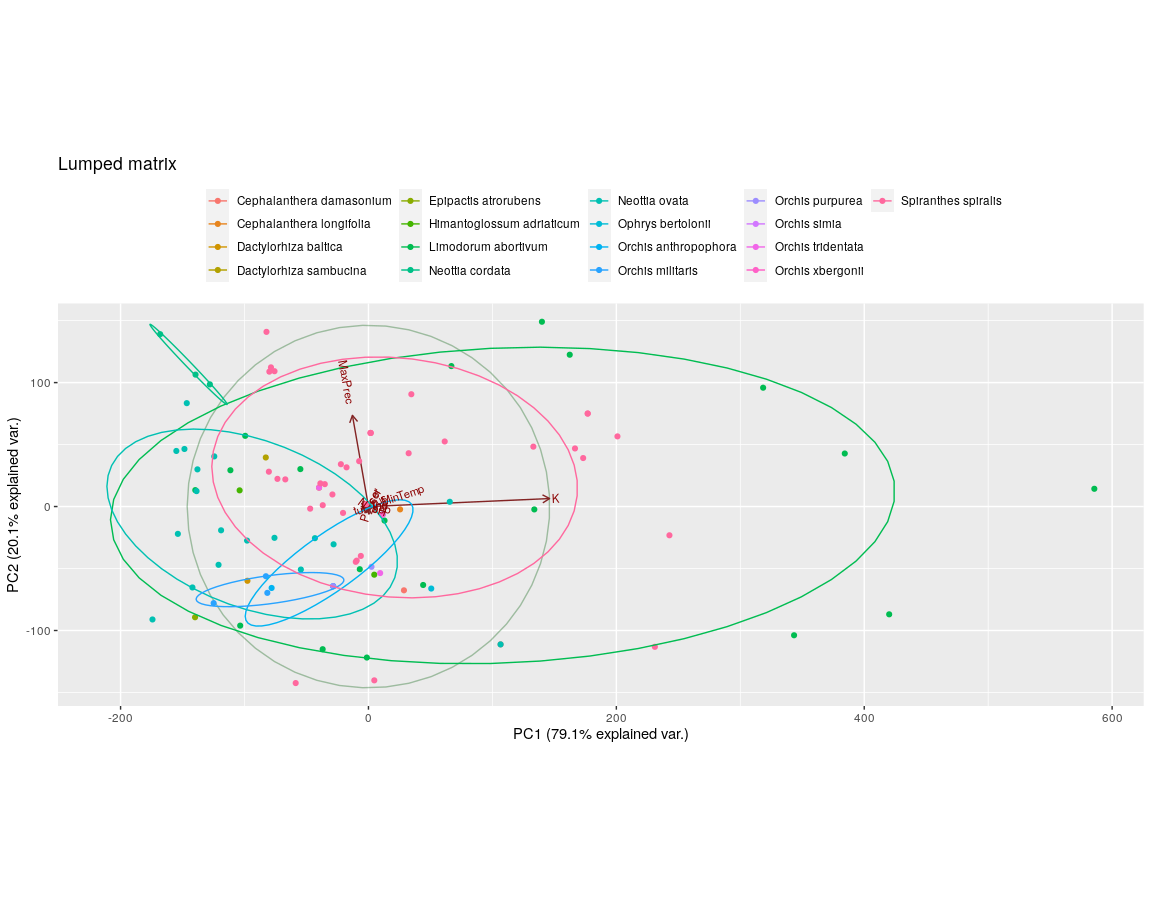
\includegraphics[keepaspectratio,width=\textwidth,height=0.75\textheight]{images/lumpPCA.png}
\caption{PCA output on of all seven OrM families}
\end{figure}

\chapter{NMDS}
\label{nmds}

The NMDS analysis on the individual OrM families seems to show that there is no differentiation in the OTUs found in different orchid species.
Again, Tulasnellaceae seem to be the exception, with more distinct groups for different orchid hosts; while this could be a bias caused by the higher number of samples, Ceratobasidiaceae and Theleophoraceae did not show this pattern even though the sample amount where roughly similar. This could point to a higher specialization of the Tulasnellaceae group, confirming previous observations ~\citep{dearnaley2007}.
The NMDS comparing the families yielded only a partial overlapping clustering, which could indicate that different orchids may have different degrees of specialization and realized niche; \emph{Limodorum abortivum} seemed to exibit the highest diversity, together with \emph{Spiranthes spiralis}.

Removing orchid species from the NMDS analysis and only looking at how different OrM families clustered based on the environmental conditions showed an unexpected pattern. Russulaceae seemed to have a high variance, which points to a broader realized niche, compared to all other families; Tulasnellaceae, which is the most sampled and abundant OrM in the dataset, had less than half the variance and clustered in an area comparable to Sebacinaceae. Stress value is close to zero (0.0003), which means that the results are robust (or that we have insufficient data).

\begin{figure}[htbp]
\centering
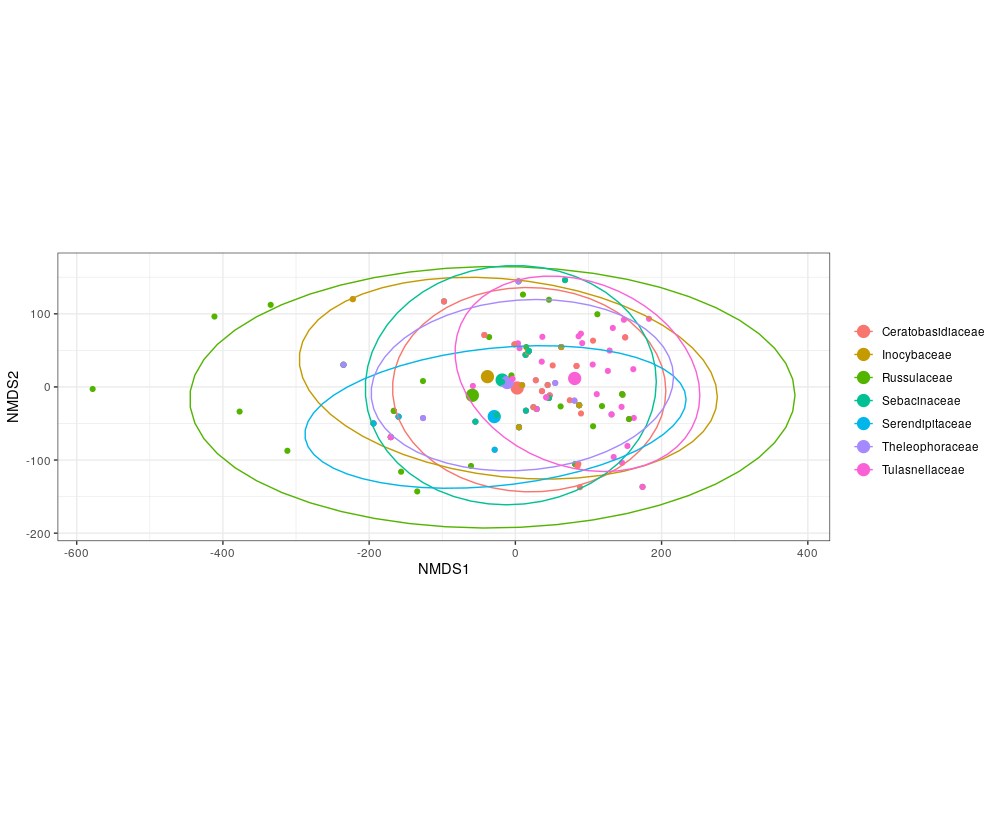
\includegraphics[keepaspectratio,width=\textwidth,height=0.75\textheight]{images/nmdsEnvMatrix.png}
\caption{NMDS output of the OrMs families considering environmental variables only}
\end{figure}

\chapter{Hierarchical modelling of species communities}
\label{hierarchicalmodellingofspeciescommunities}

The calculated Joint species distribution modelling in HMSC had a high average AUC (over 0.8), which means is robust. The AUC (Area Under the Roc Curve) provides an aggregate measure of performance across all possible classification thresholds. One way of interpreting AUC is as the probability that the model ranks a random positive example more highly than a random negative example. The AUC ranges from 0 to 1. A model whose predictions are 100\% wrong has an AUC of 0.0; one whose predictions are 100\% correct has an AUC of 1.0.

In the correlation between the families seemed like most families had a positive correlation, with two exceptions: Tulasnellaceae, who had no correlation (0) and Russulaceae, that had a negative correlation (-1). OTUs from the same families seemed, on the other hand, to have no correlation with the others, positive or negative. This remains for all families but Ceratobasidiaceae, which had more complex correlations, both positive and negative.

\begin{figure}[htbp]
\centering
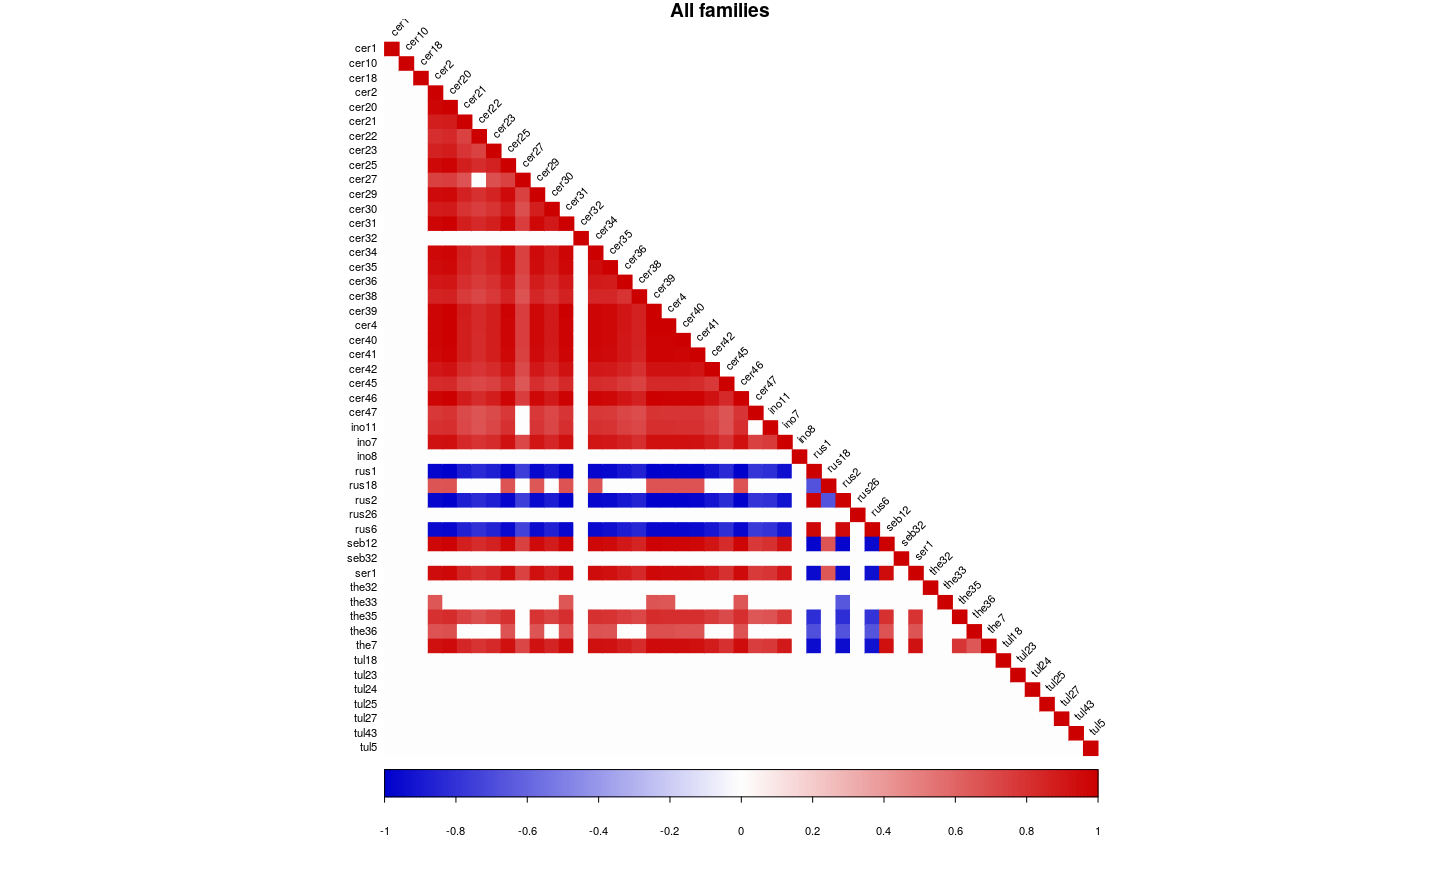
\includegraphics[keepaspectratio,width=\textwidth,height=0.75\textheight]{images/corrPlot.png}
\caption{Correlation plot between the OTUs}
\end{figure}

The second HMSC result is the correlation between the groups and the environmental variables.
The difference between the families was not very pronounced, and the most relevant parameter seemed the Minimum Temperature, which was highly correlated with most families (only Tulasnellaceae had 0 correlation), confirming the importance of this environmental parameter in understanding the distribution of OrMs. Maximum precipitation also has inverse correlation with most families, except for Russulaceae which showed a positive correlation. Of all the soil parameters, pH seemed the most important with a general inverse correlation (the lower the pH, the higher the presence of the OrM).
The differences between OTUs from the same family were less clear-cut, showing different correlations for different OTUs in the same family, giving an idea of the diversity that can happen also at low taxonomic levels.
It is worthy of notice that Tulasnellaceae showed again the least amount of internal differences.

\begin{figure}[htbp]
\centering
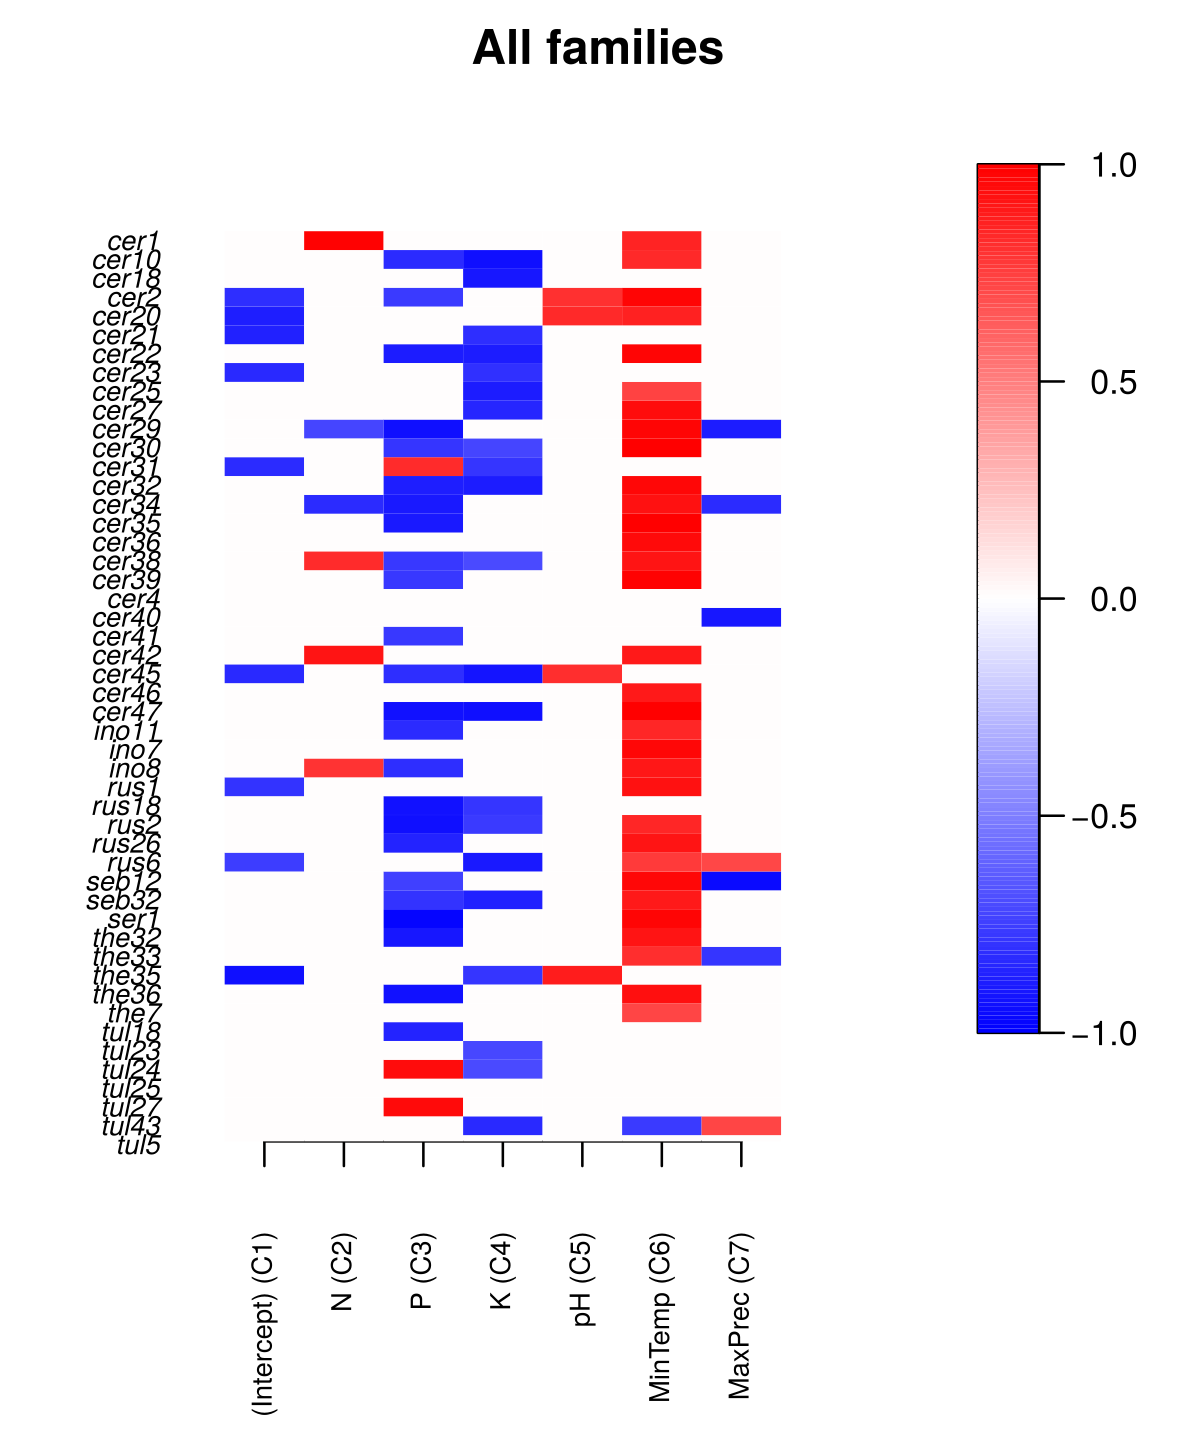
\includegraphics[keepaspectratio,width=\textwidth,height=0.75\textheight]{images/envVar.png}
\caption{HMSC output with the correlation between environmental variables and OTUs presence}
\end{figure}

The last HMSC result is how the variance of the environmental variables is distributed in each OTU. The minumum temperature of the coldest quarter usually has the higher variance

\begin{figure}[htbp]
\centering
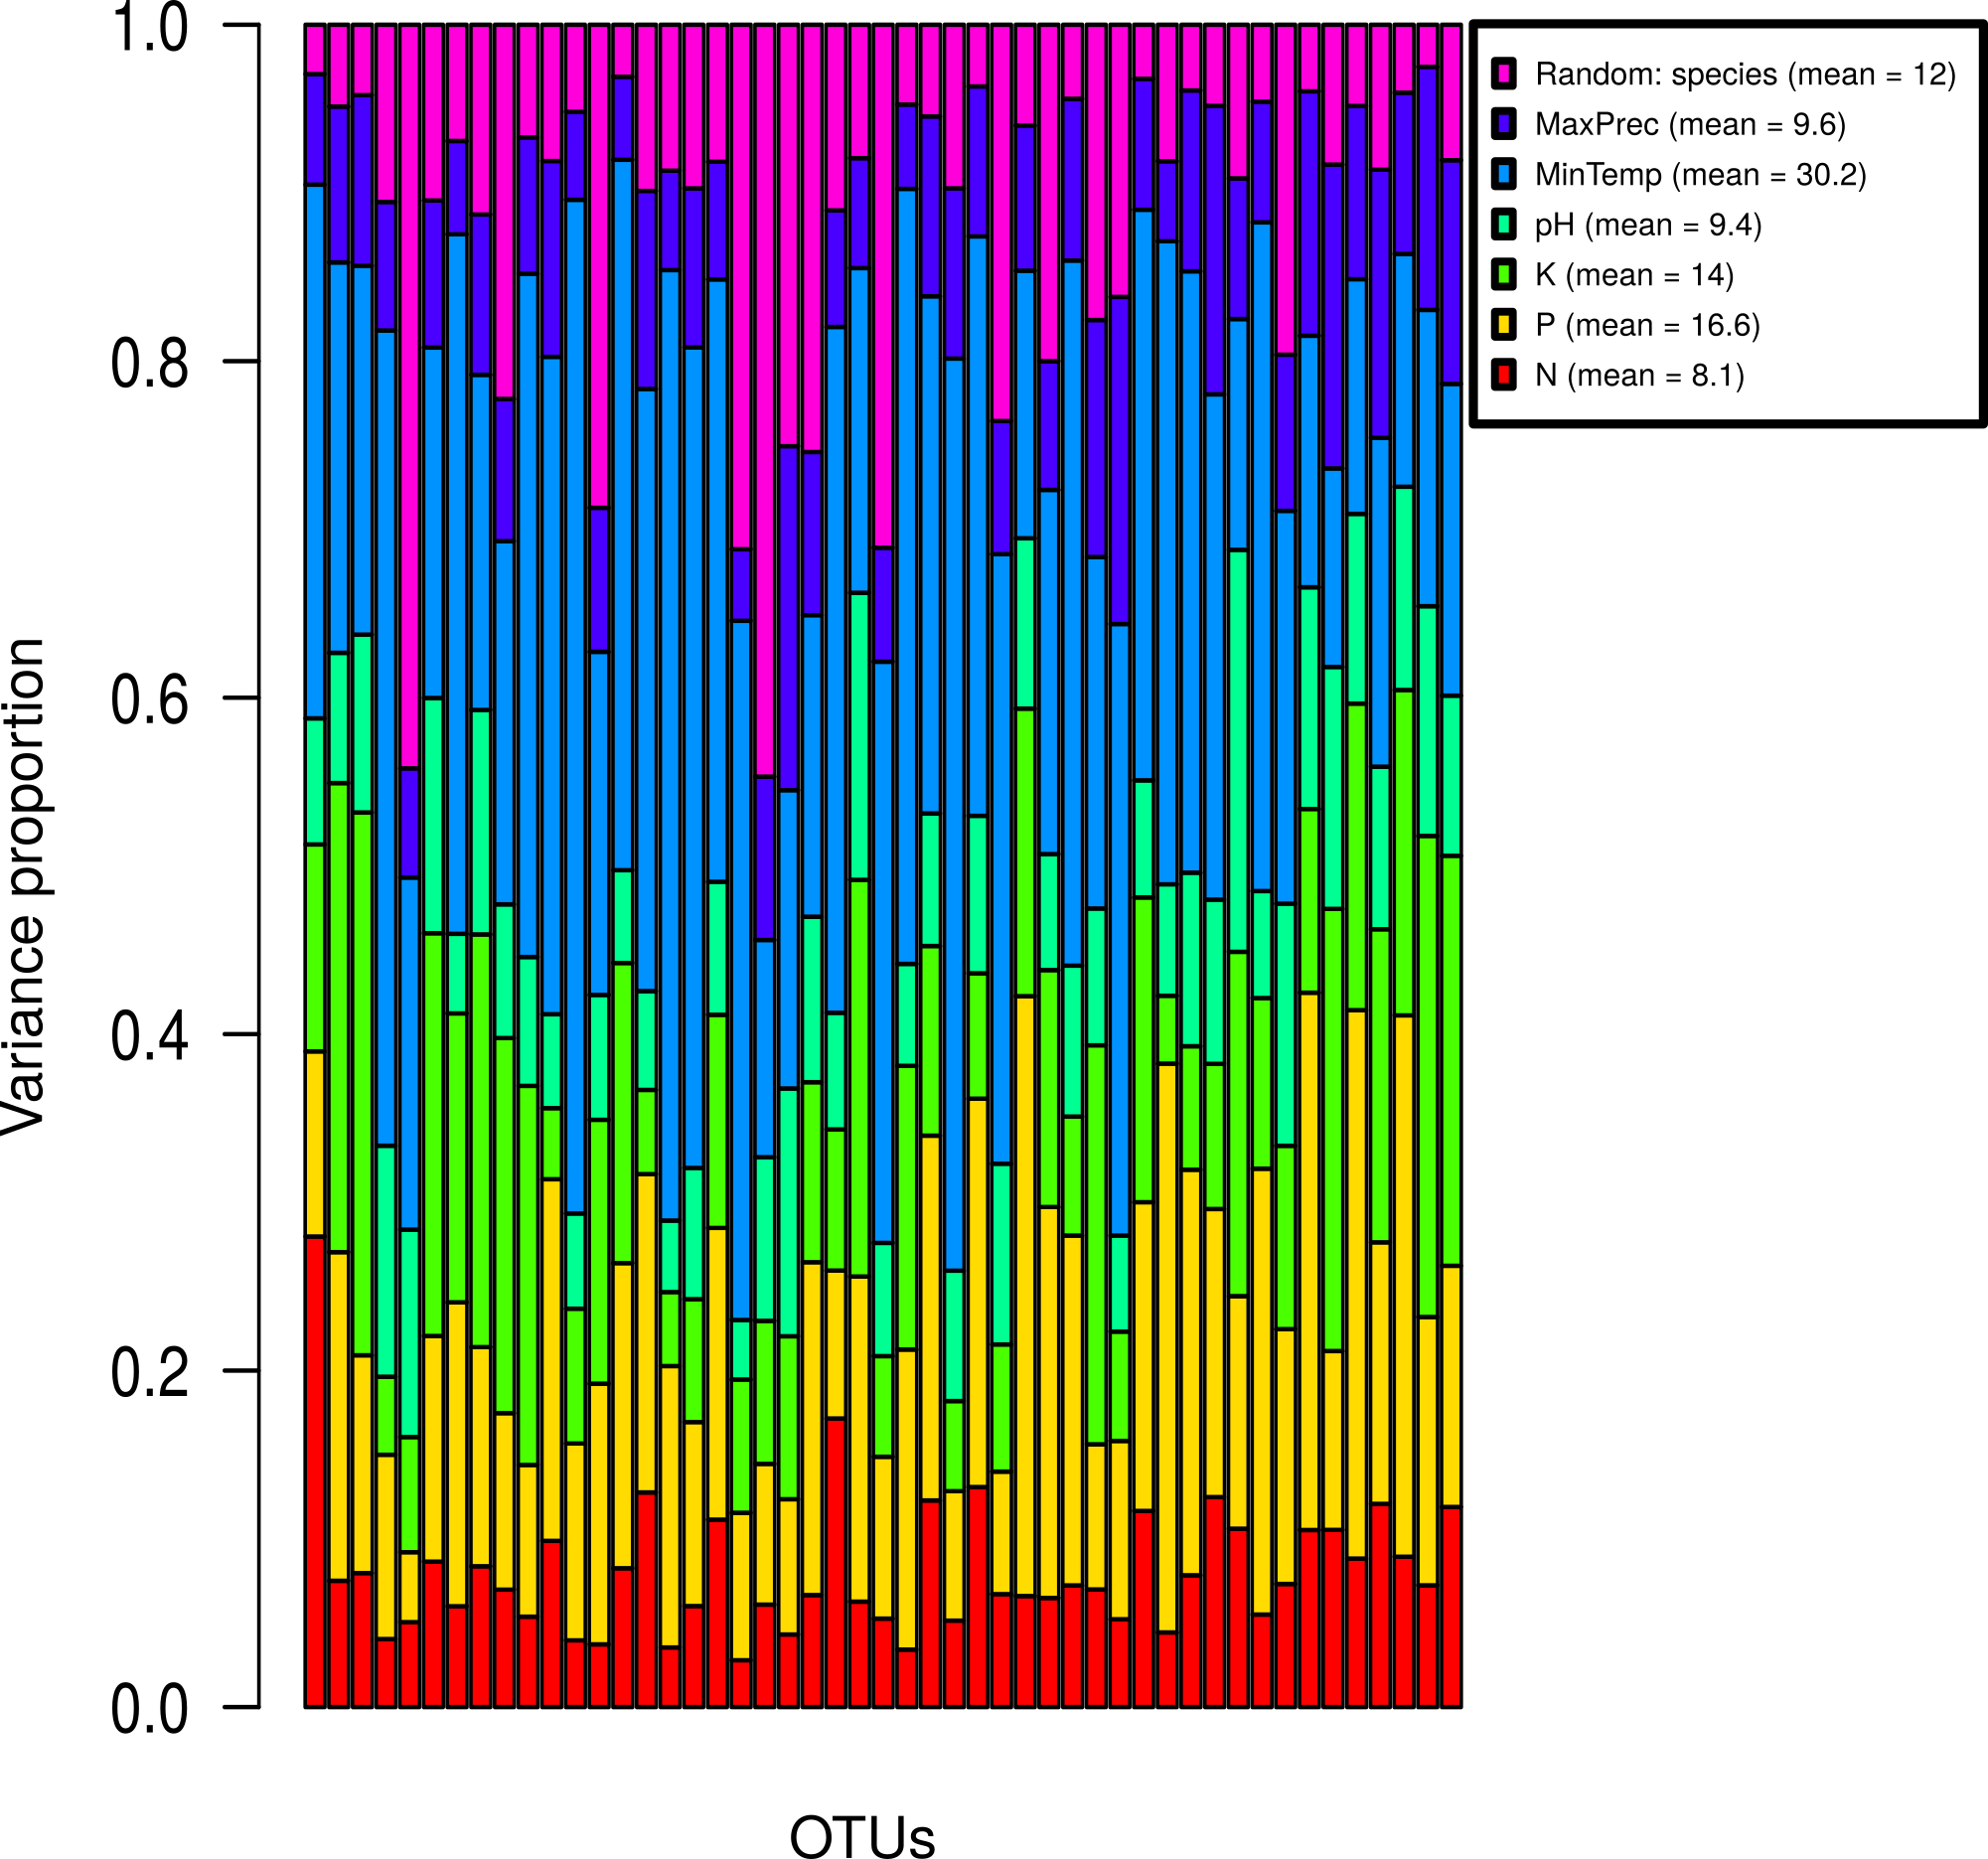
\includegraphics[keepaspectratio,width=\textwidth,height=0.75\textheight]{images/varDistribution00.png}
\caption{The relative importance (proportion of variance explained) of each fixed and random effect on the distributions of the 49 OTUs used in the HMSC analysis. OTU order follows the output of Fig. 6.}
\end{figure}

\part{Discussion}
\label{discussion}

This thesis investigated the distribution and ecological factors of OrM across Europe using a combination of phylogenetic analysis, multivariate analysis and hierarchical\slash joint species distribution modelling techniques. I found that, overall, both PCA and NMDS grouped together the OrM identified from different orchid species. This would support the idea of the OrM as being as being generalist, in that they have broad distributions, but they associate with different orchid species. The extent to which orchids have specialized or generalized relationships with OrM is a still ongoing debate ~\citep{bailarote2012}.

The phylogenetic analysis yielded low resolution results between individual OTUs from different OrM families. This was likely due to the different methods used to obtain the sequences, as the different primers allowed to polymerize different DNA areas, with only a partial overlap; this, coupled with the different trimming of the sequences done by the authors can explain the poor quality matrix that was so obtained. This piece of data would be crucial in properly understanding and framing the ecological evidence.

In the PCA most of the variance was explained by two variables, soil potassium and maximum precipitation of the wettest quarter, which means that those variables contribute the most to the definition of the niche of the OrM and that the orchids occur in places highly differentiated in those parameters. This could also be the result of the very broad sampling, and more research should be done on a smaller scale, as the potassium levels can dramatically vary even in a very small plot, often doubling in just a few meters ~\citep{bogunovic2014}.

From the NMDS Russulaceae seemed to be more tolerant than other families to different environments, and despite the lower number of sampled individuals we witness a higher variance. This could mean that the Russulaceae are more generalist toward orchids, that they have a wider niche, that it's more ecologically flexible, it was sampled in a broader area or all of the above. Russulaceae are a very diverse family, but it is actually difficult to say that Russulaceae find a ``niche'' in the symbiosis with orchids, especially with Limodorum, as there doesn't seem to be any advantage for the fungus: this orchids seem to have an insufficient photosynthesis and to heavily rely on the OrM to provide not only minerals but also carbon-base chemicals; this also means that distribution of Limodorum may also be potentially constrained by the occurrence of its fungal symbionts ~\citep{girlanda2005}.

Inocybaceae have a high variance too, probably because of the few sampled points (eleven); this is in contrast with more sampled OrM families, such as Tulasnellaceae and Ceratobasidiaceae, which show the lowest amount of variance, explainable by a more specialist niche, for the families themselves or for the orchids that host them. Serendipitaceae have a very low number of samples (two), but show nonetheless a variance comparable to the mean of all the families.

The HMSC analysis showed clearly that there are residual correlations between OrM taxa. To my knowledge, this shows for the first time that OrM have ecological interactions beyond what is explained by environmental variables. Members of Ceratobasidiaceae tend to have positive residual correlations among them, that is, is likely Ceratobasidiaceae OTUs to co-occur. In some other cases, there is a zero correlation, so they do not influence each other's presence. This is interesting as the most broadly sampled orchid included in this study, \emph{Spiranthes spiralis}, is predominately associated with OTUs of Ceratobasidiaceae. It could be that the positive residual co-occurrence are the result of facilitation between taxa of Ceratobasidiaceae, which may in turn positively affect orchid occurrence at a particular site.
Inocybaceae, Sebacinaceae and Theleophoraceae show similar results but less pronounced, either because residual correlation was not as strong (as in the Theleophoraceae) or because the positive correlation trend is not as common.

In contrast with the Ceratobasidiaceae trend, and in accordance with the multivariate analyses, the residual co-occurrence of members of Russulaceae were mostly negatively correlated with the other families. This means that where we find Russulaceae, we are unlikely going to find other OrM, of any family. This is probably the result of the main orchid species where Russulas were found in this dataset, \emph{Limodorum abortivum}, which seems to show a specialization toward this family ~\citep{girlanda2005}. A single OTU, identified as \emph{rus18} in the present work, showed a general positive correlation also with other families.

Tulasnellaceae shows no residual correlations at all (zero) either between other OTUs of the same OrM family, or with OTUs of different families.

The correlation between OrM and environmental variables in the HMSC model showed some shared patterns. Most of the OrM were positive correlated with the minimum temperature of the coldest quarter, in all families except Tulasnellaceae, which had a zero correlation (except for a single OTU, \emph{tul5}). Two other trends stand out: the phosphorus and potassium soil content, which are generally negatively correlated with little exceptions.
Nitrogen is often considered a major community changer in the soil fungal communities, ~\citep{lilleskov2002} both because of the nitrogen itself and because it's considered a proxy to infer human impact, especially for agricultural reason. The model, however, show little correlation between the OrM and the soil nitrogen content, which could be explained as evidence of the little impact of nitrogen on the communities or as evidence of communities already changed in their composition by the nutrients content by selection, so that the resulting OrM are not as impacted.
The pH level was of little relevance, and so was the maximum precipitation, the reason for which should be subject of future studies, but it could be the effect of the limited sample size.

Variance partitioning for each OTUs of all the environmental values shows how for some variables there is a relevant difference between the OTUs, especially for the random effect (which was associated with the host orchid). Soil nitrogen and the maximum precipitation variable seem to vary the least, which is in line with the correlation plot: they are not good predictors of the kind of OrM that we could find in a place. Potassium and phosphorus have a higher relative variance.
This variables could therefore be considered the most useful in understanding the distribution of OrM, and may be a good starting point for further niche modelling.

The phylogenetic analysis didn't give significative results. This was likely due to the different methods used to obtain the sequences, as the different primers allowed to polymerize different DNA areas, with only a partial overlap; this, coupled with the different trimming of the sequences done by the authors can explain the poor quality matrix that was so obtained.
This piece of data would be crucial in properly understanding and framing the ecological evidence.

Do similar OrM taxa occur in similar habitats and have similar environmental preferences? Some taxa do, and in the same family there are shared correlations for environmental variables from the HMSC, while the NMDS analysis shows a narrow ecological niche with shared correlation to environmental variables in some families, e.g. Tulasnellaceae, Ceratobasidiaceae, Theleophoraceae, and a broader niche in others, in particular Russulaceae and Inocybaceae. This seems to be irrespective of the sample size.

The correlation between the OTUs presence is quite robust, so there may be facilitation or competition processes happening between the OrM. Further studies are required to understand what the nature of these processes are, how much the OrM themselves are responsable for it and what is the importance of the orchid host in the process. It is also important to notice that the sampled orchids were of unknown age, likely adult as those are easier to sample. We do know that orchids change preferences for the fungal symbiont through life, and the ones identified in an adult plant are not necessarily those that will allow the seed to germinate ~\citep{meng2019}, making those findings difficult to apply in a conservation plan.

These kind of studies are important for the understanding and protection of taxa that are not yet described. As I investigated OTUs in this study, it is not clear whether these taxa are true species. Improving soil ecosystem health is not something we can successfully do without knowing the key elements that allow important taxa such as fungi to function. Presently there is limited georeferenced studies that allow the pinpointing of mycorrhizal fungi in general to specific locations, resulting difficulty in performing analyses such as presented in this thesis. The understanding of OrM ecology will always be incomplete without a better knowledge of the taxonomy of OrM. We lack a robust phylogenetic framework that allows adequate assessment of the phylogenetic relationships between fungal strains. This would need to start from a species concept for OrM ~\citep{jacquemyn2017}. Without this knowledge, we have limited ability to shed light on the evolutionary history of these OrM groups.

\part{Conclusions}
\label{conclusions}

In this thesis I compiled and analysed an extensive database of mycorrhizal fungi that associate with European orchids. These results show that fungi are generally associated with individual orchid species, but that members of each OrM family often occur in a broad range of ecological conditions. Competitive and facilitative interactions may be common within OrM, and this study provides a platform for future experimental work. The use of hierarchical distribution models in this thesis was a useful instrument to untangle the correlation between the OTUs and the environmental variables, and I have little doubt that in the future more work will be done using these tools.

These kind of studies are of crucial importance for the understanding and protection of species we may not even know yet. Improving the ecosystem is not something we can successfully do without knowing the key elements that allow them to function, and fungi surely are part of this category. These studies are heavily reliant on data, which must be accurate and abundant. Presently there is limited properly georeferenced studies that allow the pinpointing of genetic sequences to places, resulting in gappy databases and in a difficulty reproducing the analysis.
Furthermore, gathering the data the way I've done is mostly a manual process, with huge cost in terms of time and resources. More transparent analysis with an accessible, standardize and rich metadata structure are of the uttermost importance for a significant progress of knowledge in the understanding of ecology and distribution of OrM ~\citep{powers2019}, and for scientific studies in general.

The understanding of OrM ecology will always be incomplete without a better knowledge of the taxonomy of OrM. We lack an acceptable phylogenetic framework that allows adequate assessment of the phylogenetic relationships between fungal strains. This would need to start from a robust species concept for OrM ~\citep{jacquemyn2017}. Without this knowledge, patterns may emerge from analysis but we can't infer them to groups or use them to shed light on the evolutionary history of the groups.

It is also important to notice that the sampled orchids were of unknown age, likely adult as those are easier to sample. We do know that orchids change preferences for the fungal symbiont through life, and the ones identified in an adult plant are not necessarily those that will allow the seed to germinate ~\citep{meng2019}, making those findings difficult to apply in a conservation plan.

\part{Appendices}
\label{appendices}

\chapter{Appendix I: Additional resources and information}
\label{appendixi:additionalresourcesandinformation}

All of the datasets, scripts and resources to reproduce the analysis are available at https:\slash \slash github.com\slash arteteco\slash FunModels

Unless differently specified, the present work copyright is held by Manuel Moscariello (manuel@arteteco.com) and is released under the Creative Commons Attribution 4.0 International License. To view a copy of this license, visit http:\slash \slash creativecommons.org\slash licenses\slash by\slash 4.0\slash  or send a letter to Creative Commons, PO Box 1866, Mountain View, CA 94042, USA.

The logo of the university in the frontispiece is trademark by Università degli Studi di Napoli Federico II - Corso Umberto I 40 - 80138 Napoli (contactcenter@unina.it, PEC: ateneo@pec.unina.it)

Base satellite map on page 16 is ©2021 TerraMetrics, Map data ©2021GeoBasis-DE\slash BKG (©2009), Google, Inst Geogr. Nacional

\chapter{Appendix II: Analysis results}
\label{appendixii:analysisresults}

The following graphs are the phylogenetic trees, NMDS and PCA plots

\begin{figure}[htbp]
\centering
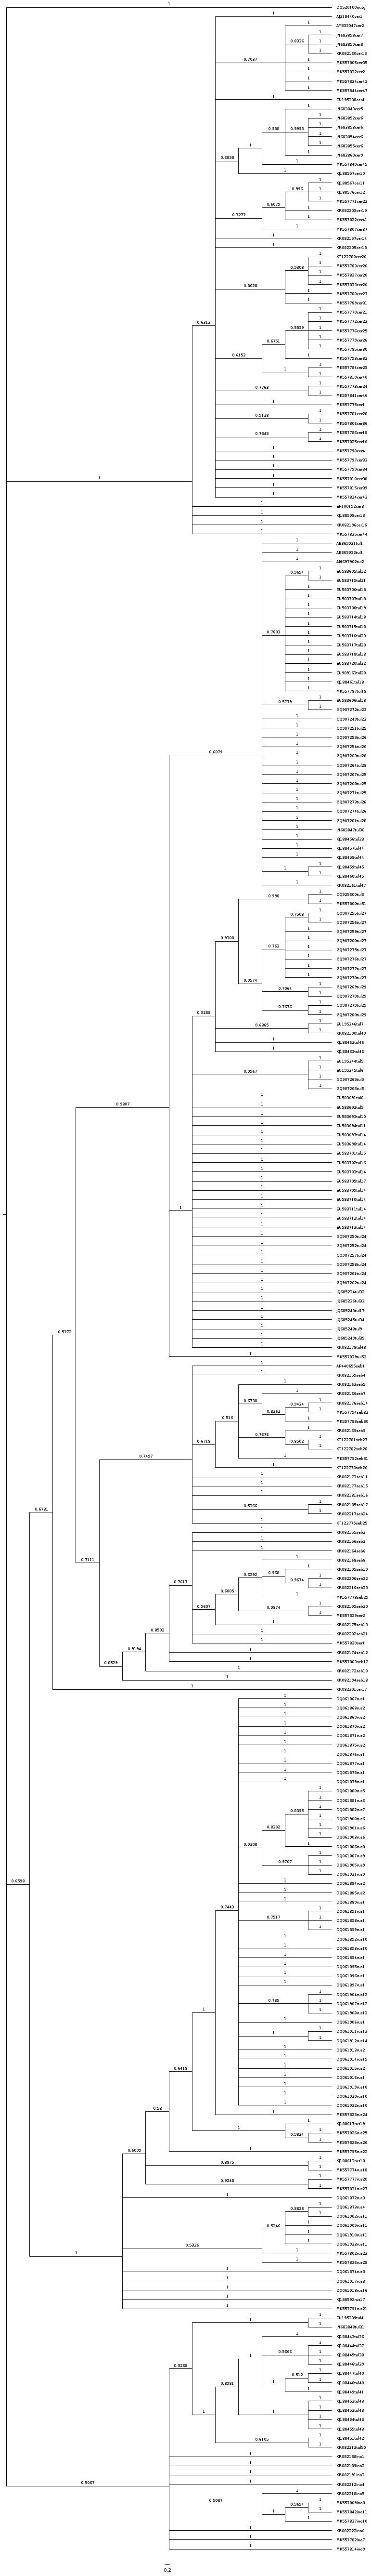
\includegraphics[keepaspectratio,width=\textwidth,height=0.75\textheight]{images/mcmc.jpg}
\caption{Bayesian analysis tree}
\end{figure}

\begin{figure}[htbp]
\centering
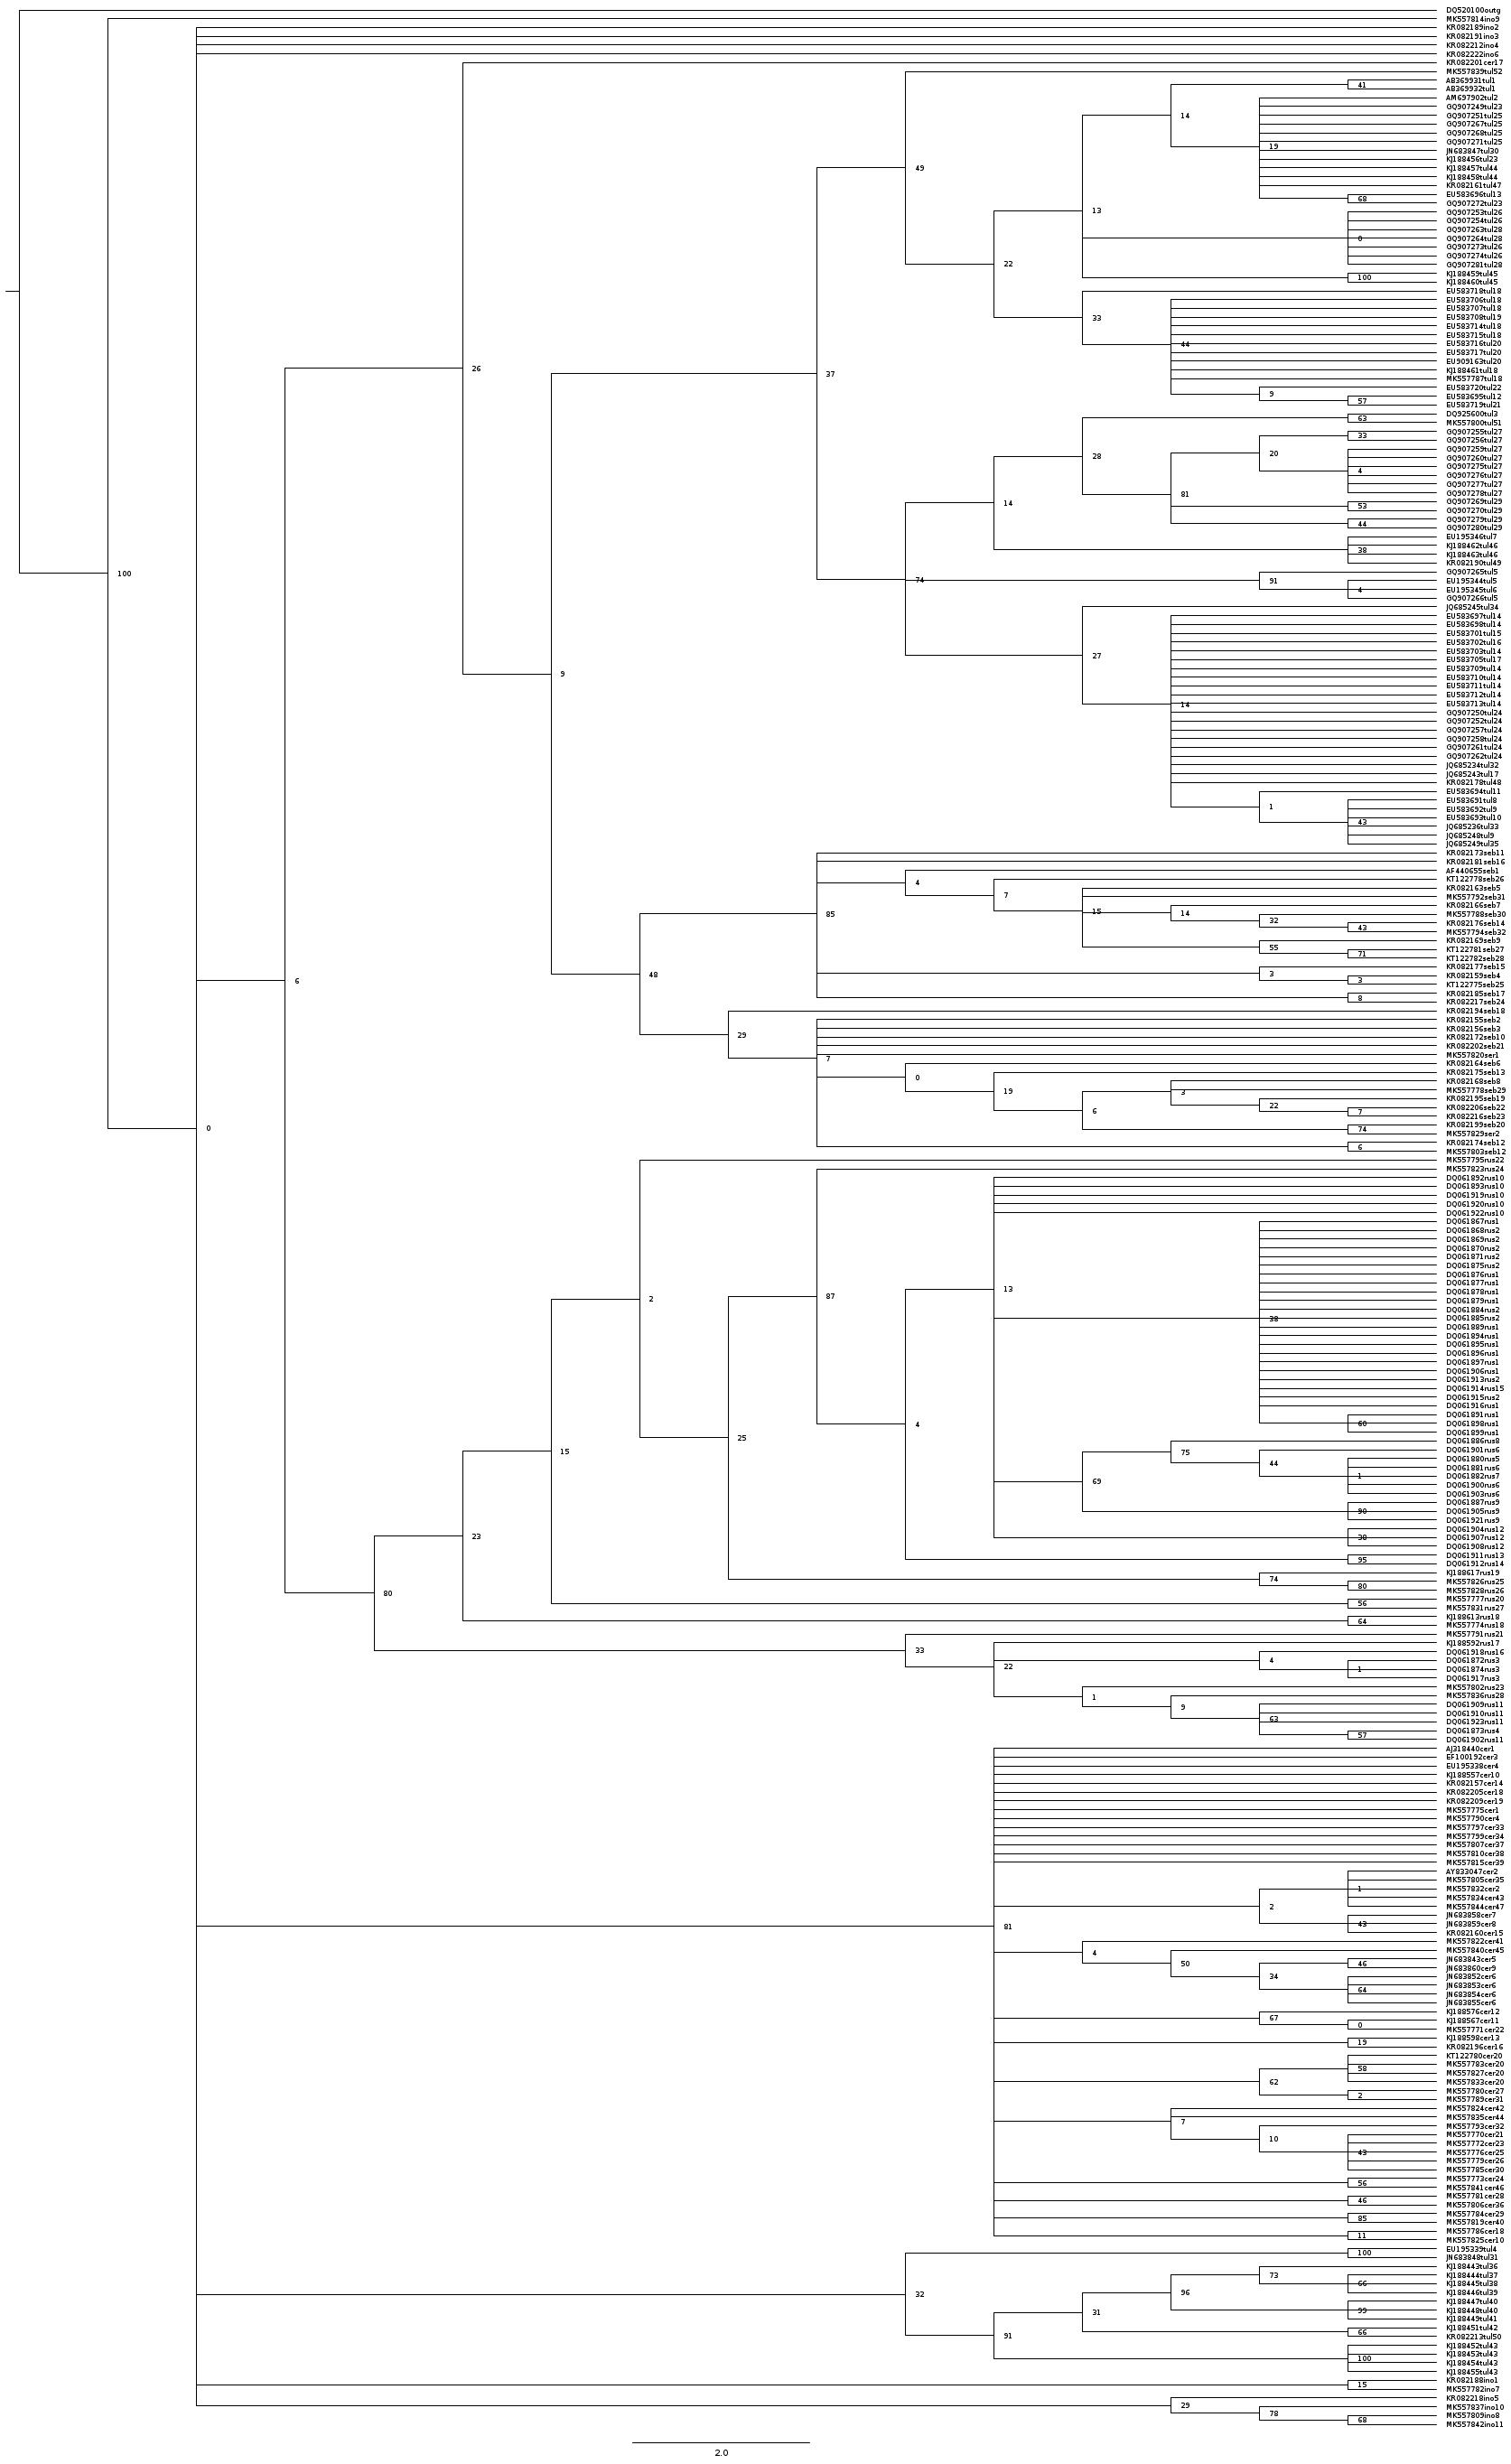
\includegraphics[keepaspectratio,width=\textwidth,height=0.75\textheight]{images/mp.jpg}
\caption{Maximum Parsimony tree. Node labels are the bootstrap values}
\end{figure}

\begin{figure}[htbp]
\centering
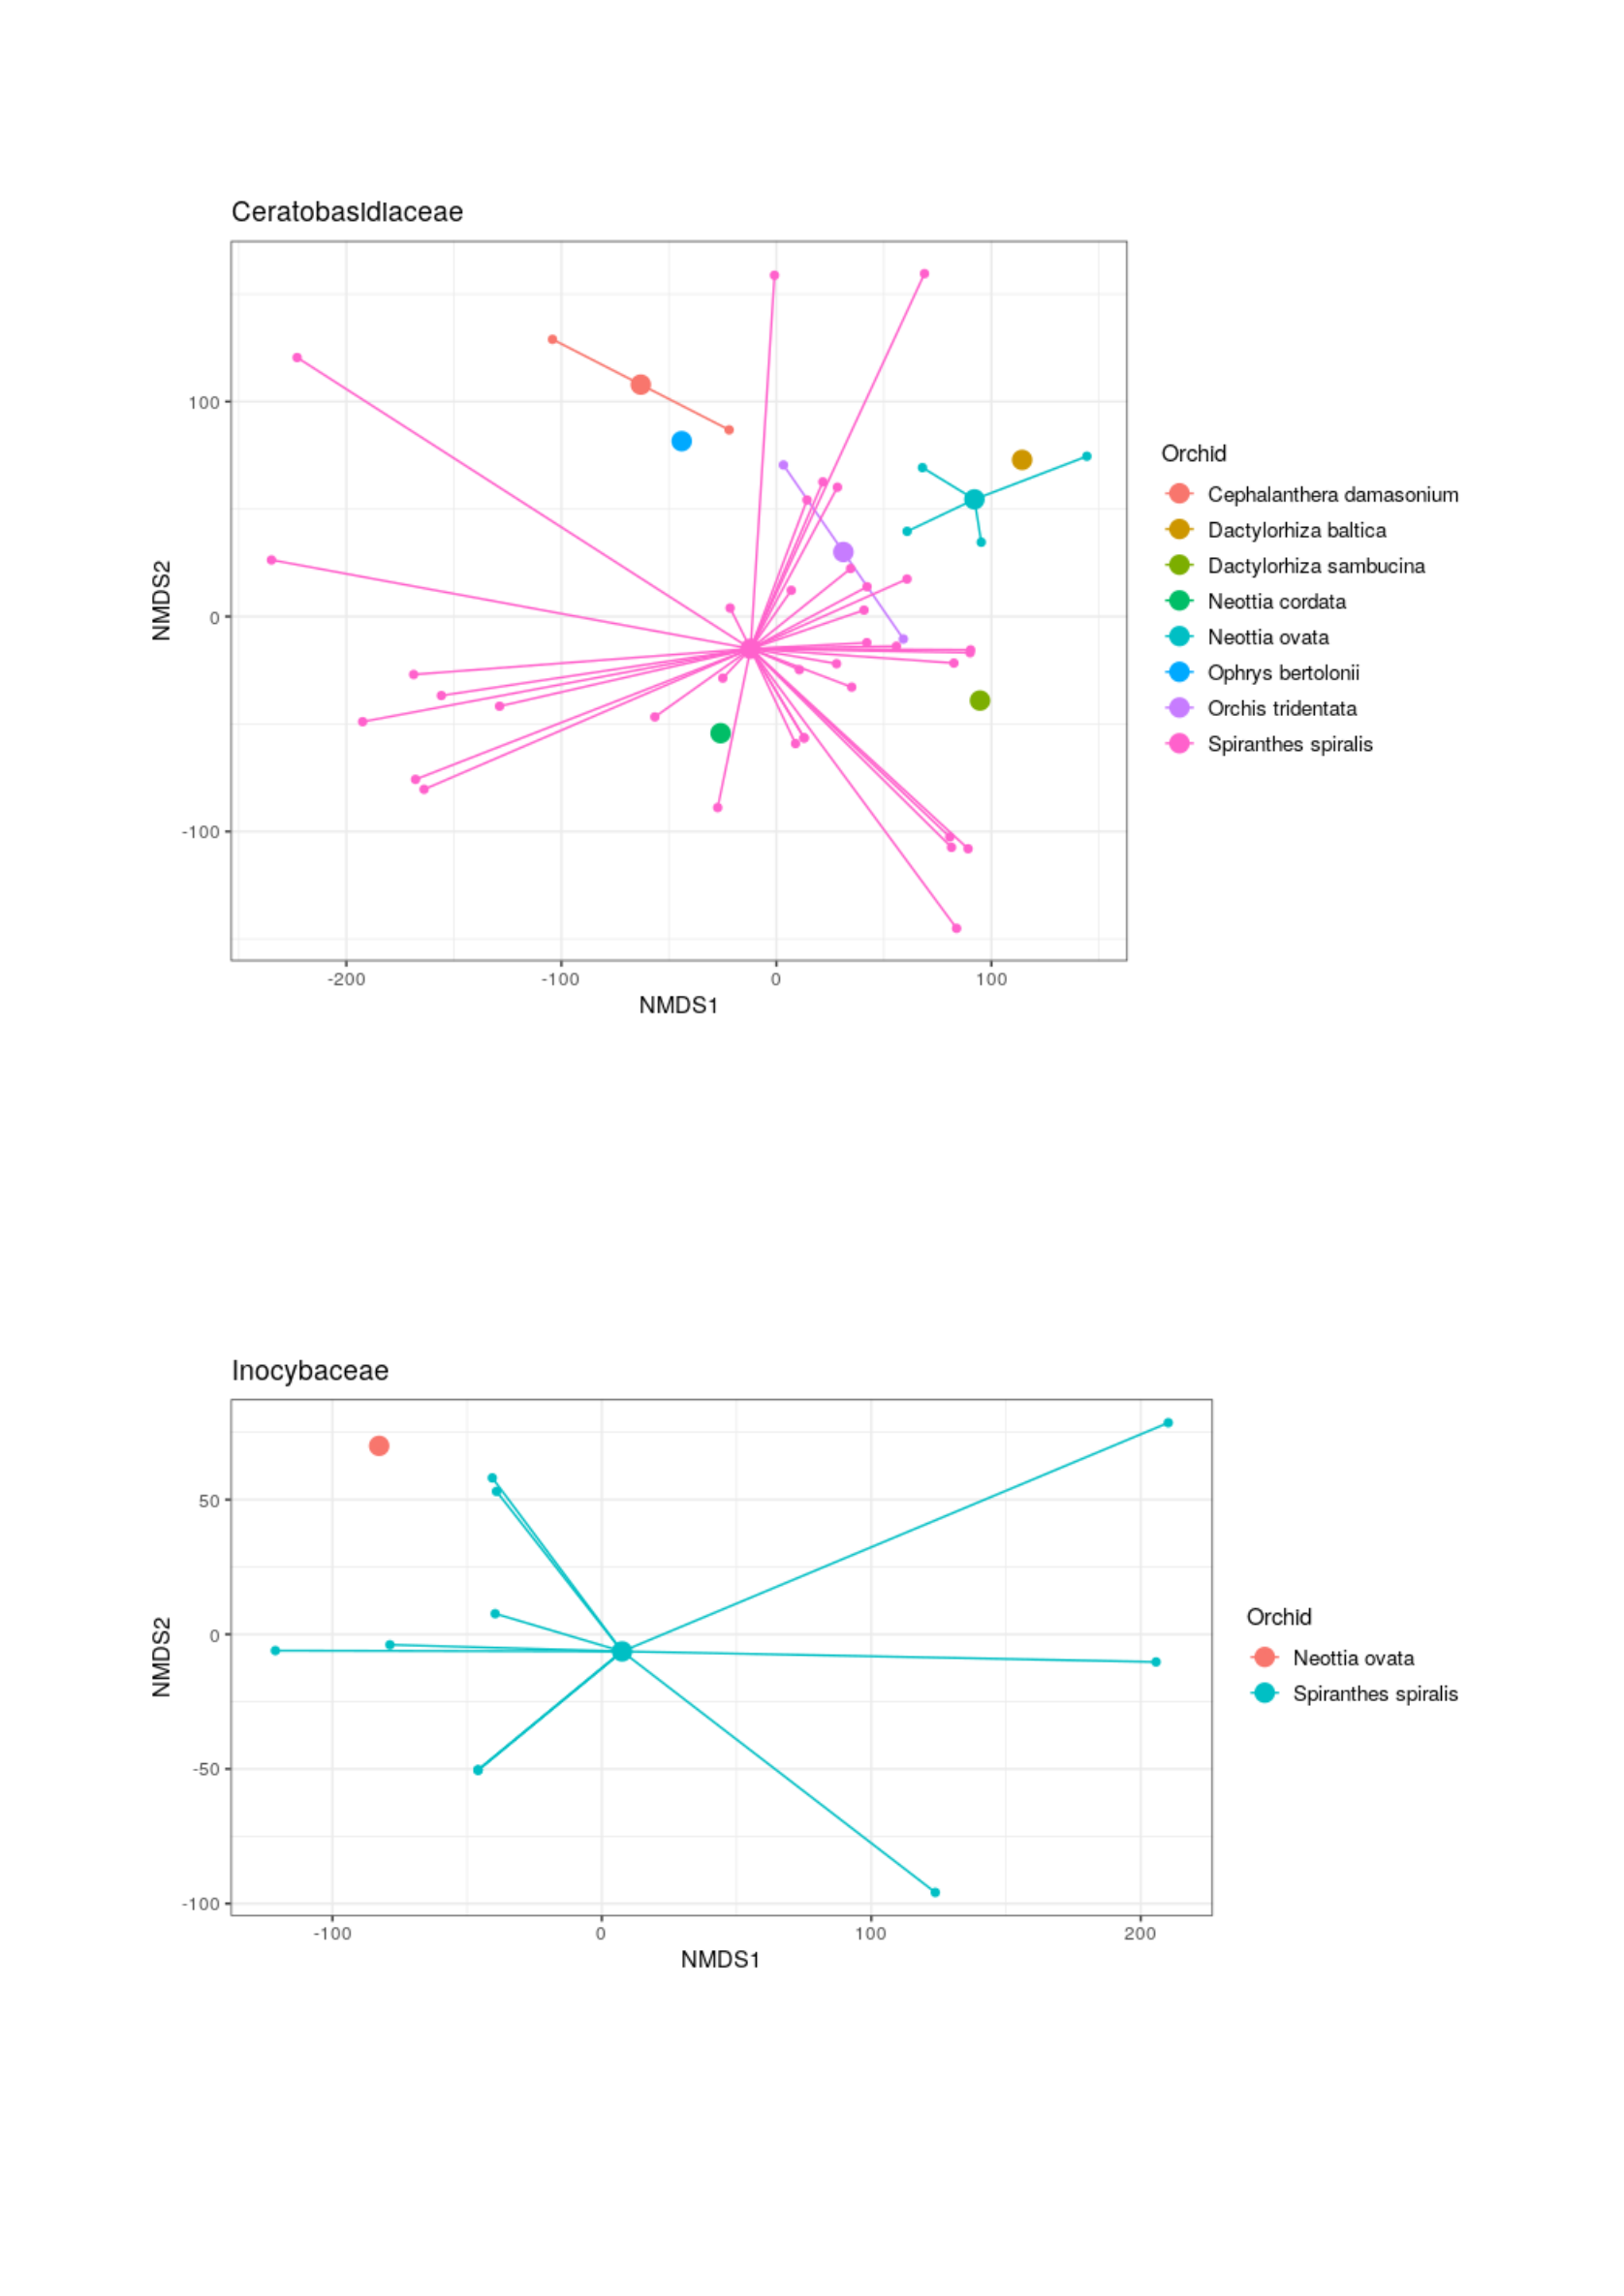
\includegraphics[keepaspectratio,width=\textwidth,height=0.75\textheight]{images/NMDScerino.png}
\caption{NMDS of Ceratobasidiaceae and Inocybaceae}
\end{figure}

\begin{figure}[htbp]
\centering
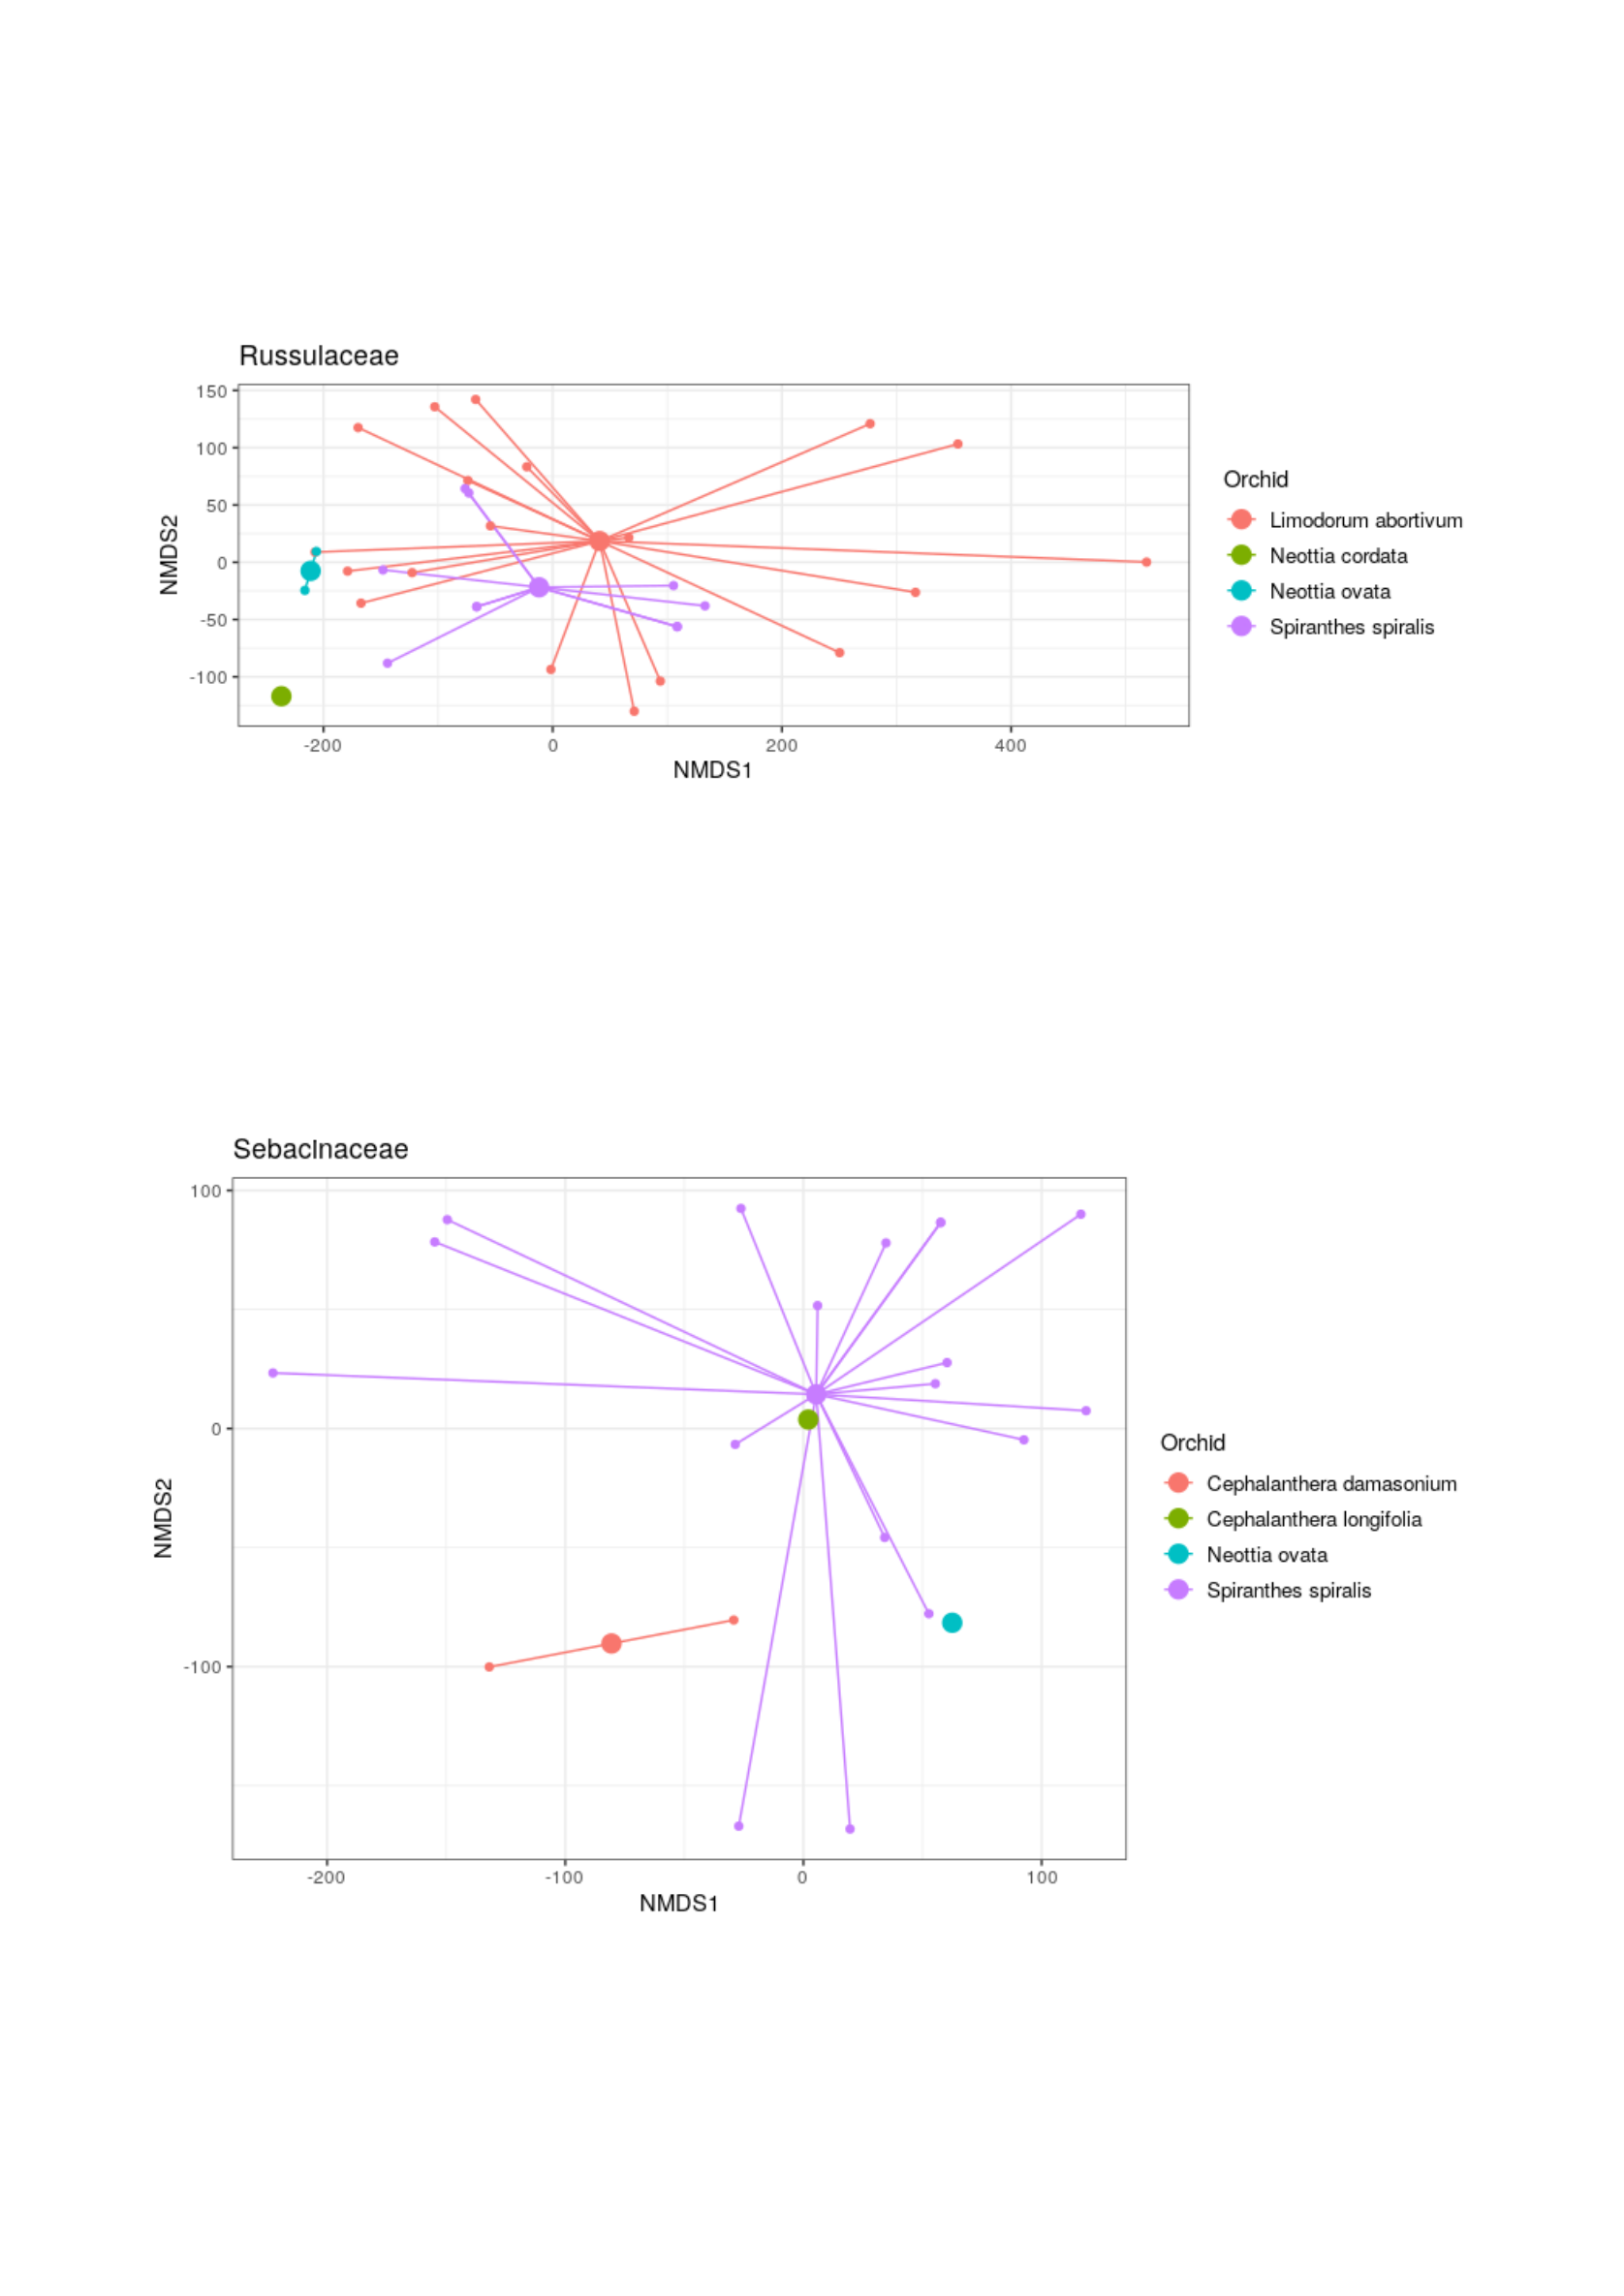
\includegraphics[keepaspectratio,width=\textwidth,height=0.75\textheight]{images/NMDSrusseb.png}
\caption{NMDS of Russulaceae and Sebacinaceae}
\end{figure}

\begin{figure}[htbp]
\centering
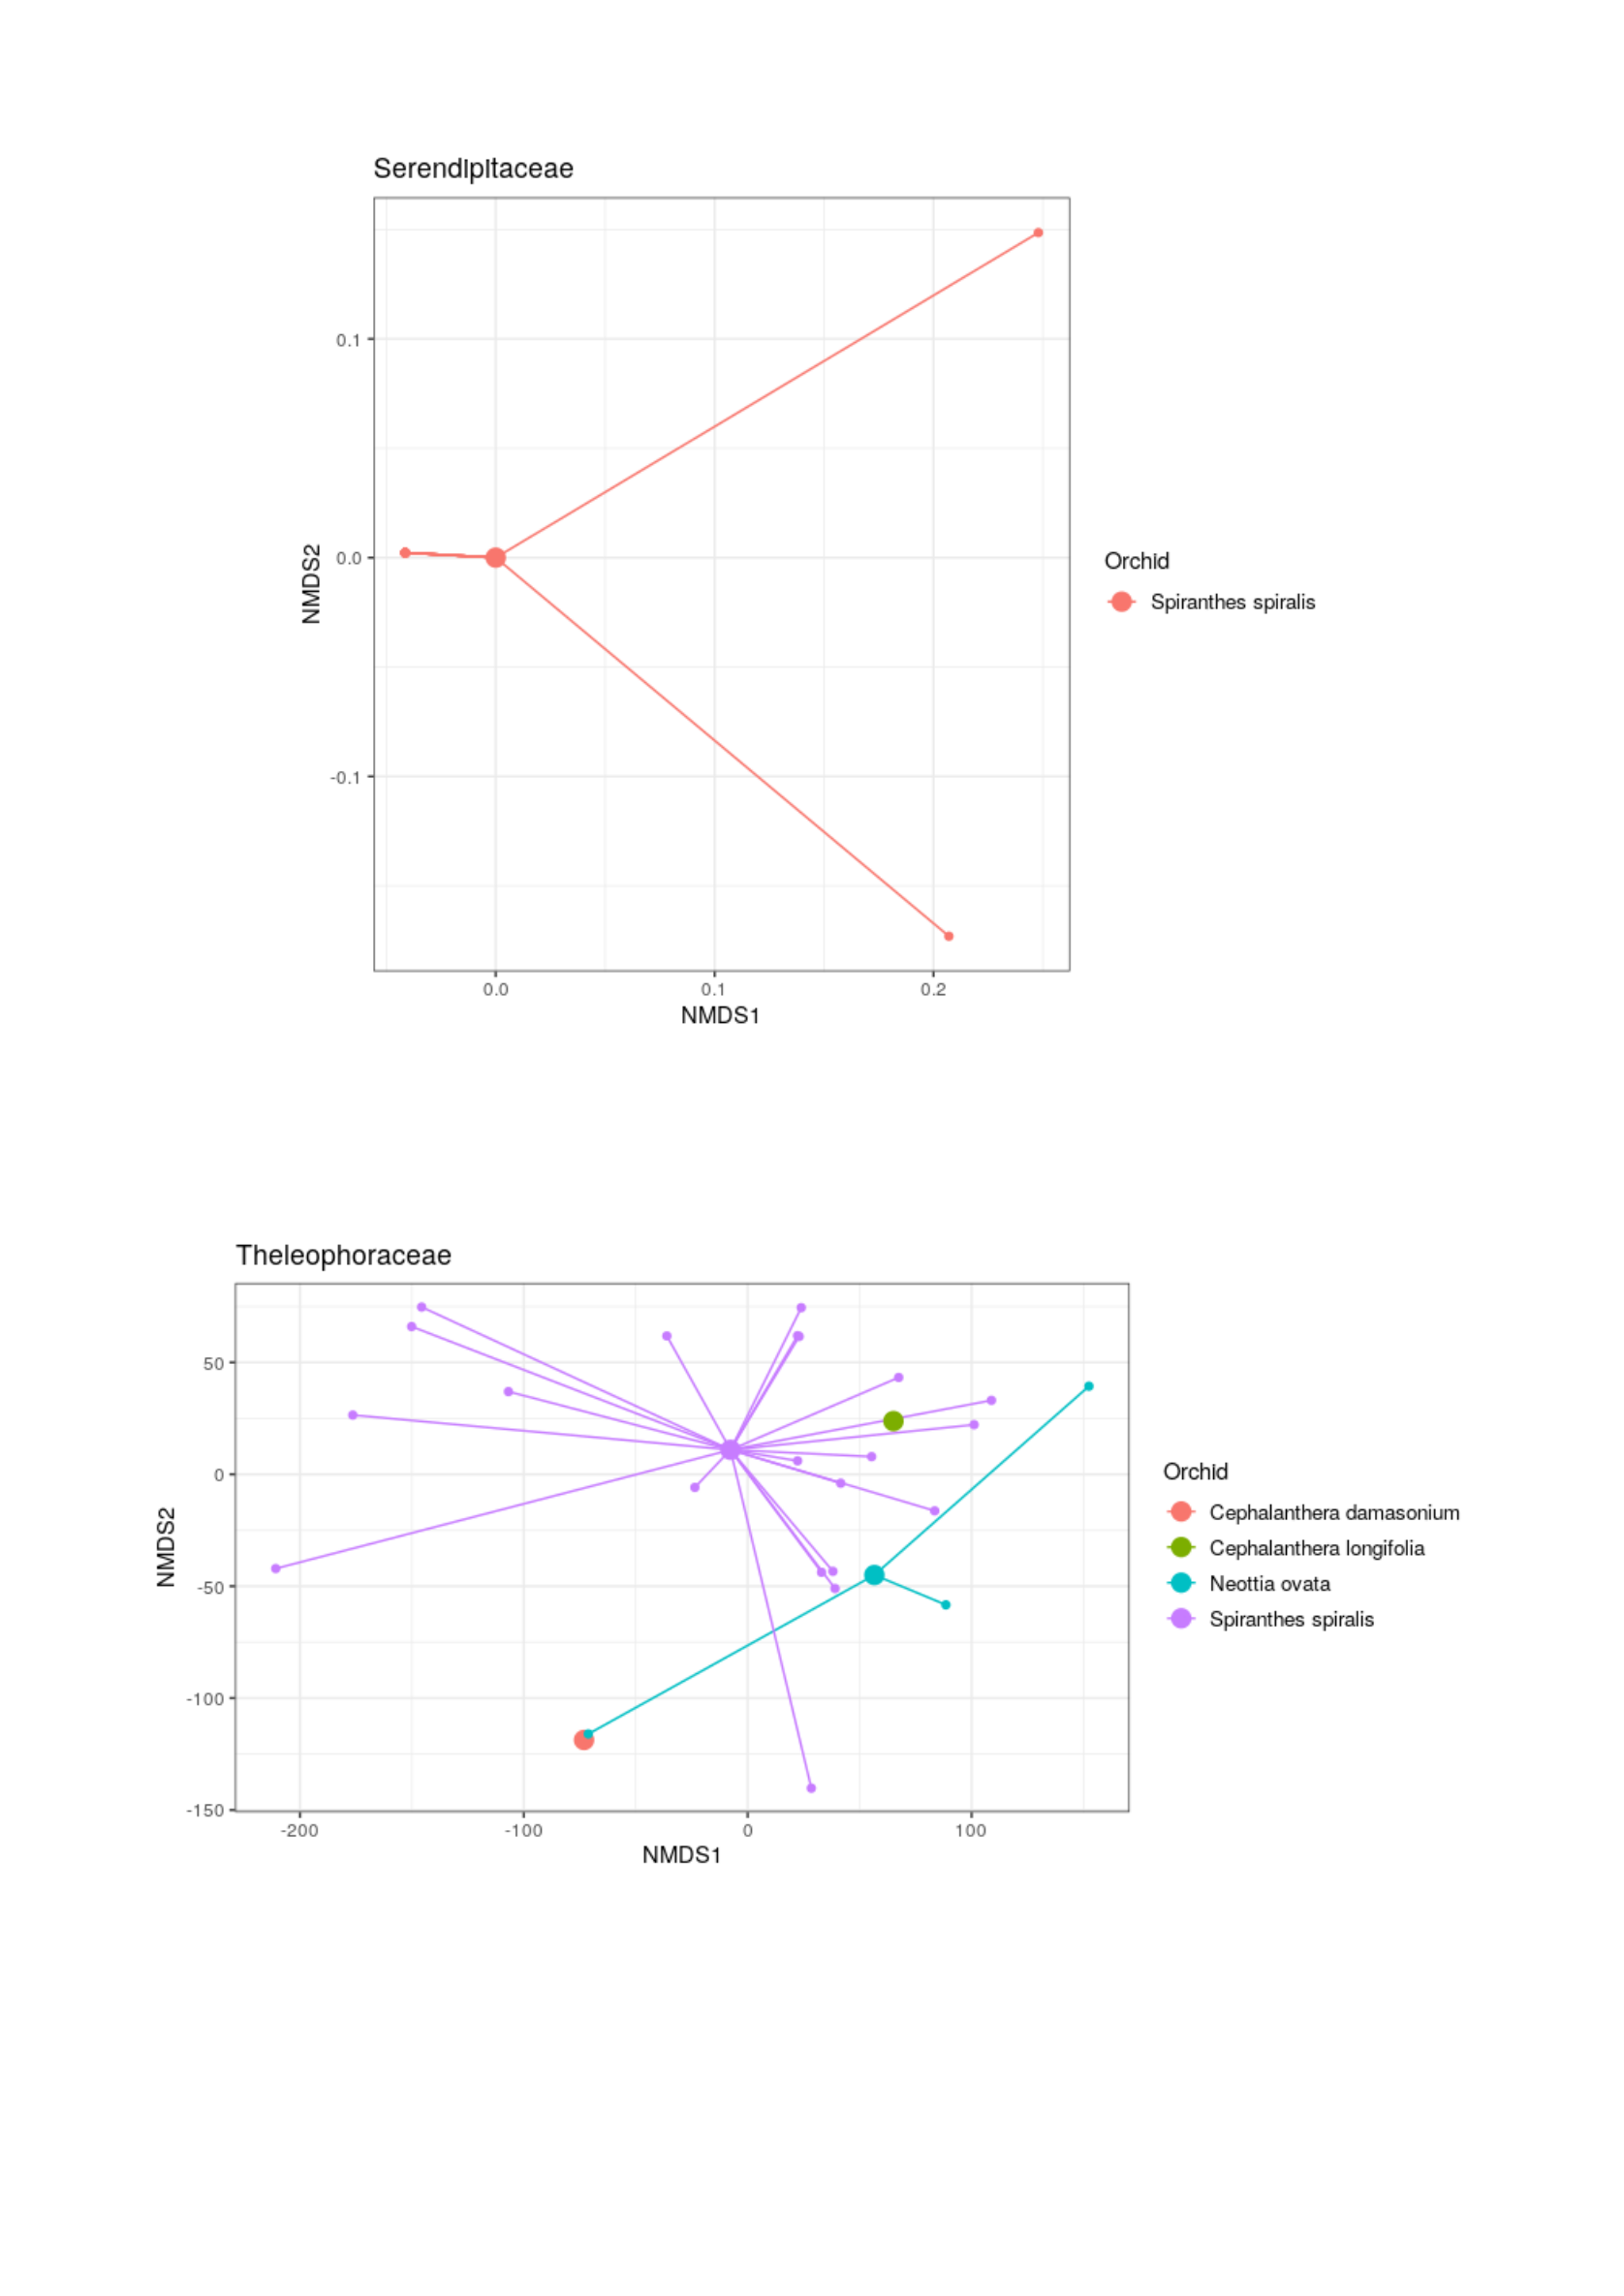
\includegraphics[keepaspectratio,width=\textwidth,height=0.75\textheight]{images/NMDSserthe.png}
\caption{NMDS of Serendipitaceae and Theleophoraceae}
\end{figure}

\begin{figure}[htbp]
\centering
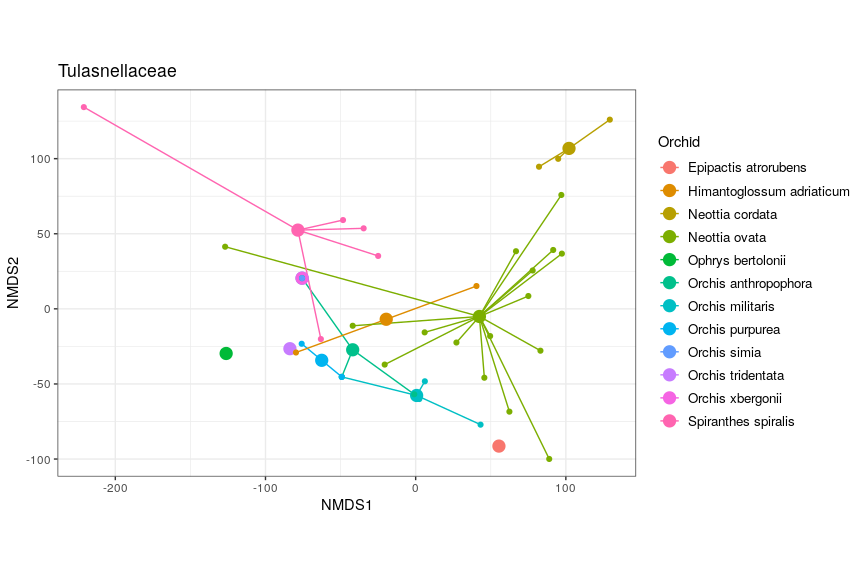
\includegraphics[keepaspectratio,width=\textwidth,height=0.75\textheight]{images/NMDStul.png}
\caption{NMDS of Tulasnellaceae}
\end{figure}

\begin{figure}[htbp]
\centering
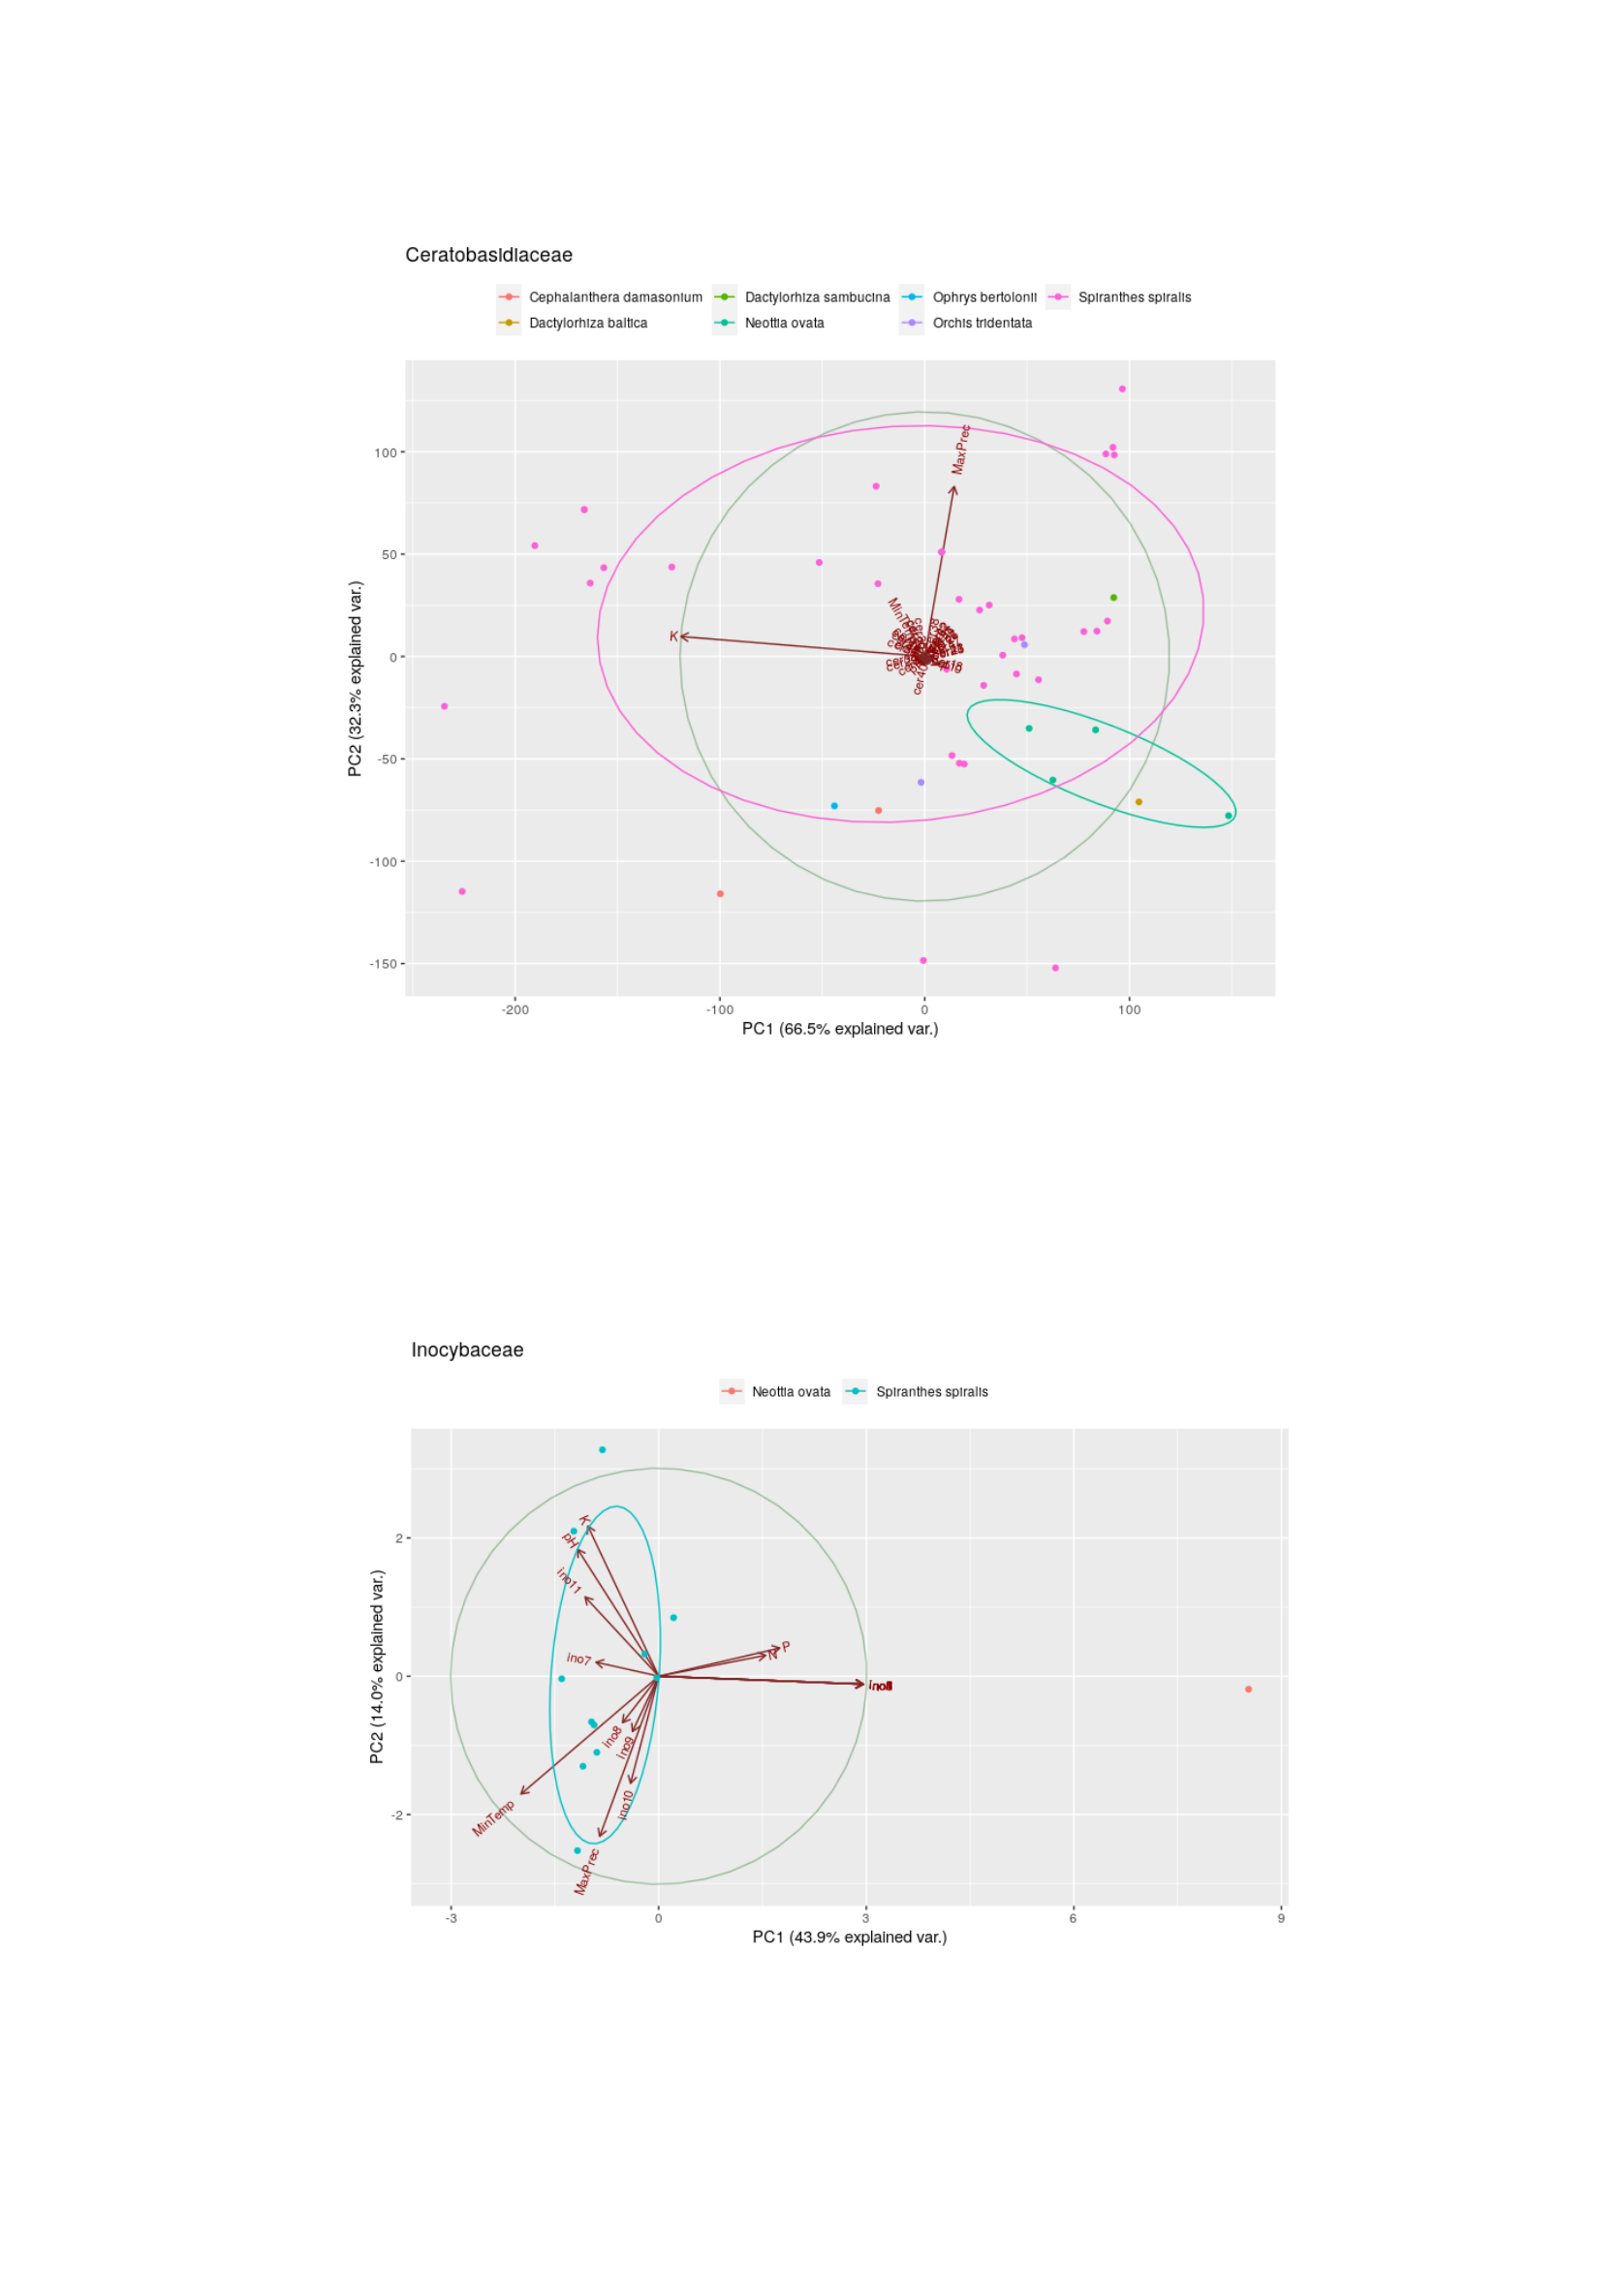
\includegraphics[keepaspectratio,width=\textwidth,height=0.75\textheight]{images/PCAcerino.png}
\caption{PCA of Ceratobasidiaceae and Inocybaceae}
\end{figure}

\begin{figure}[htbp]
\centering
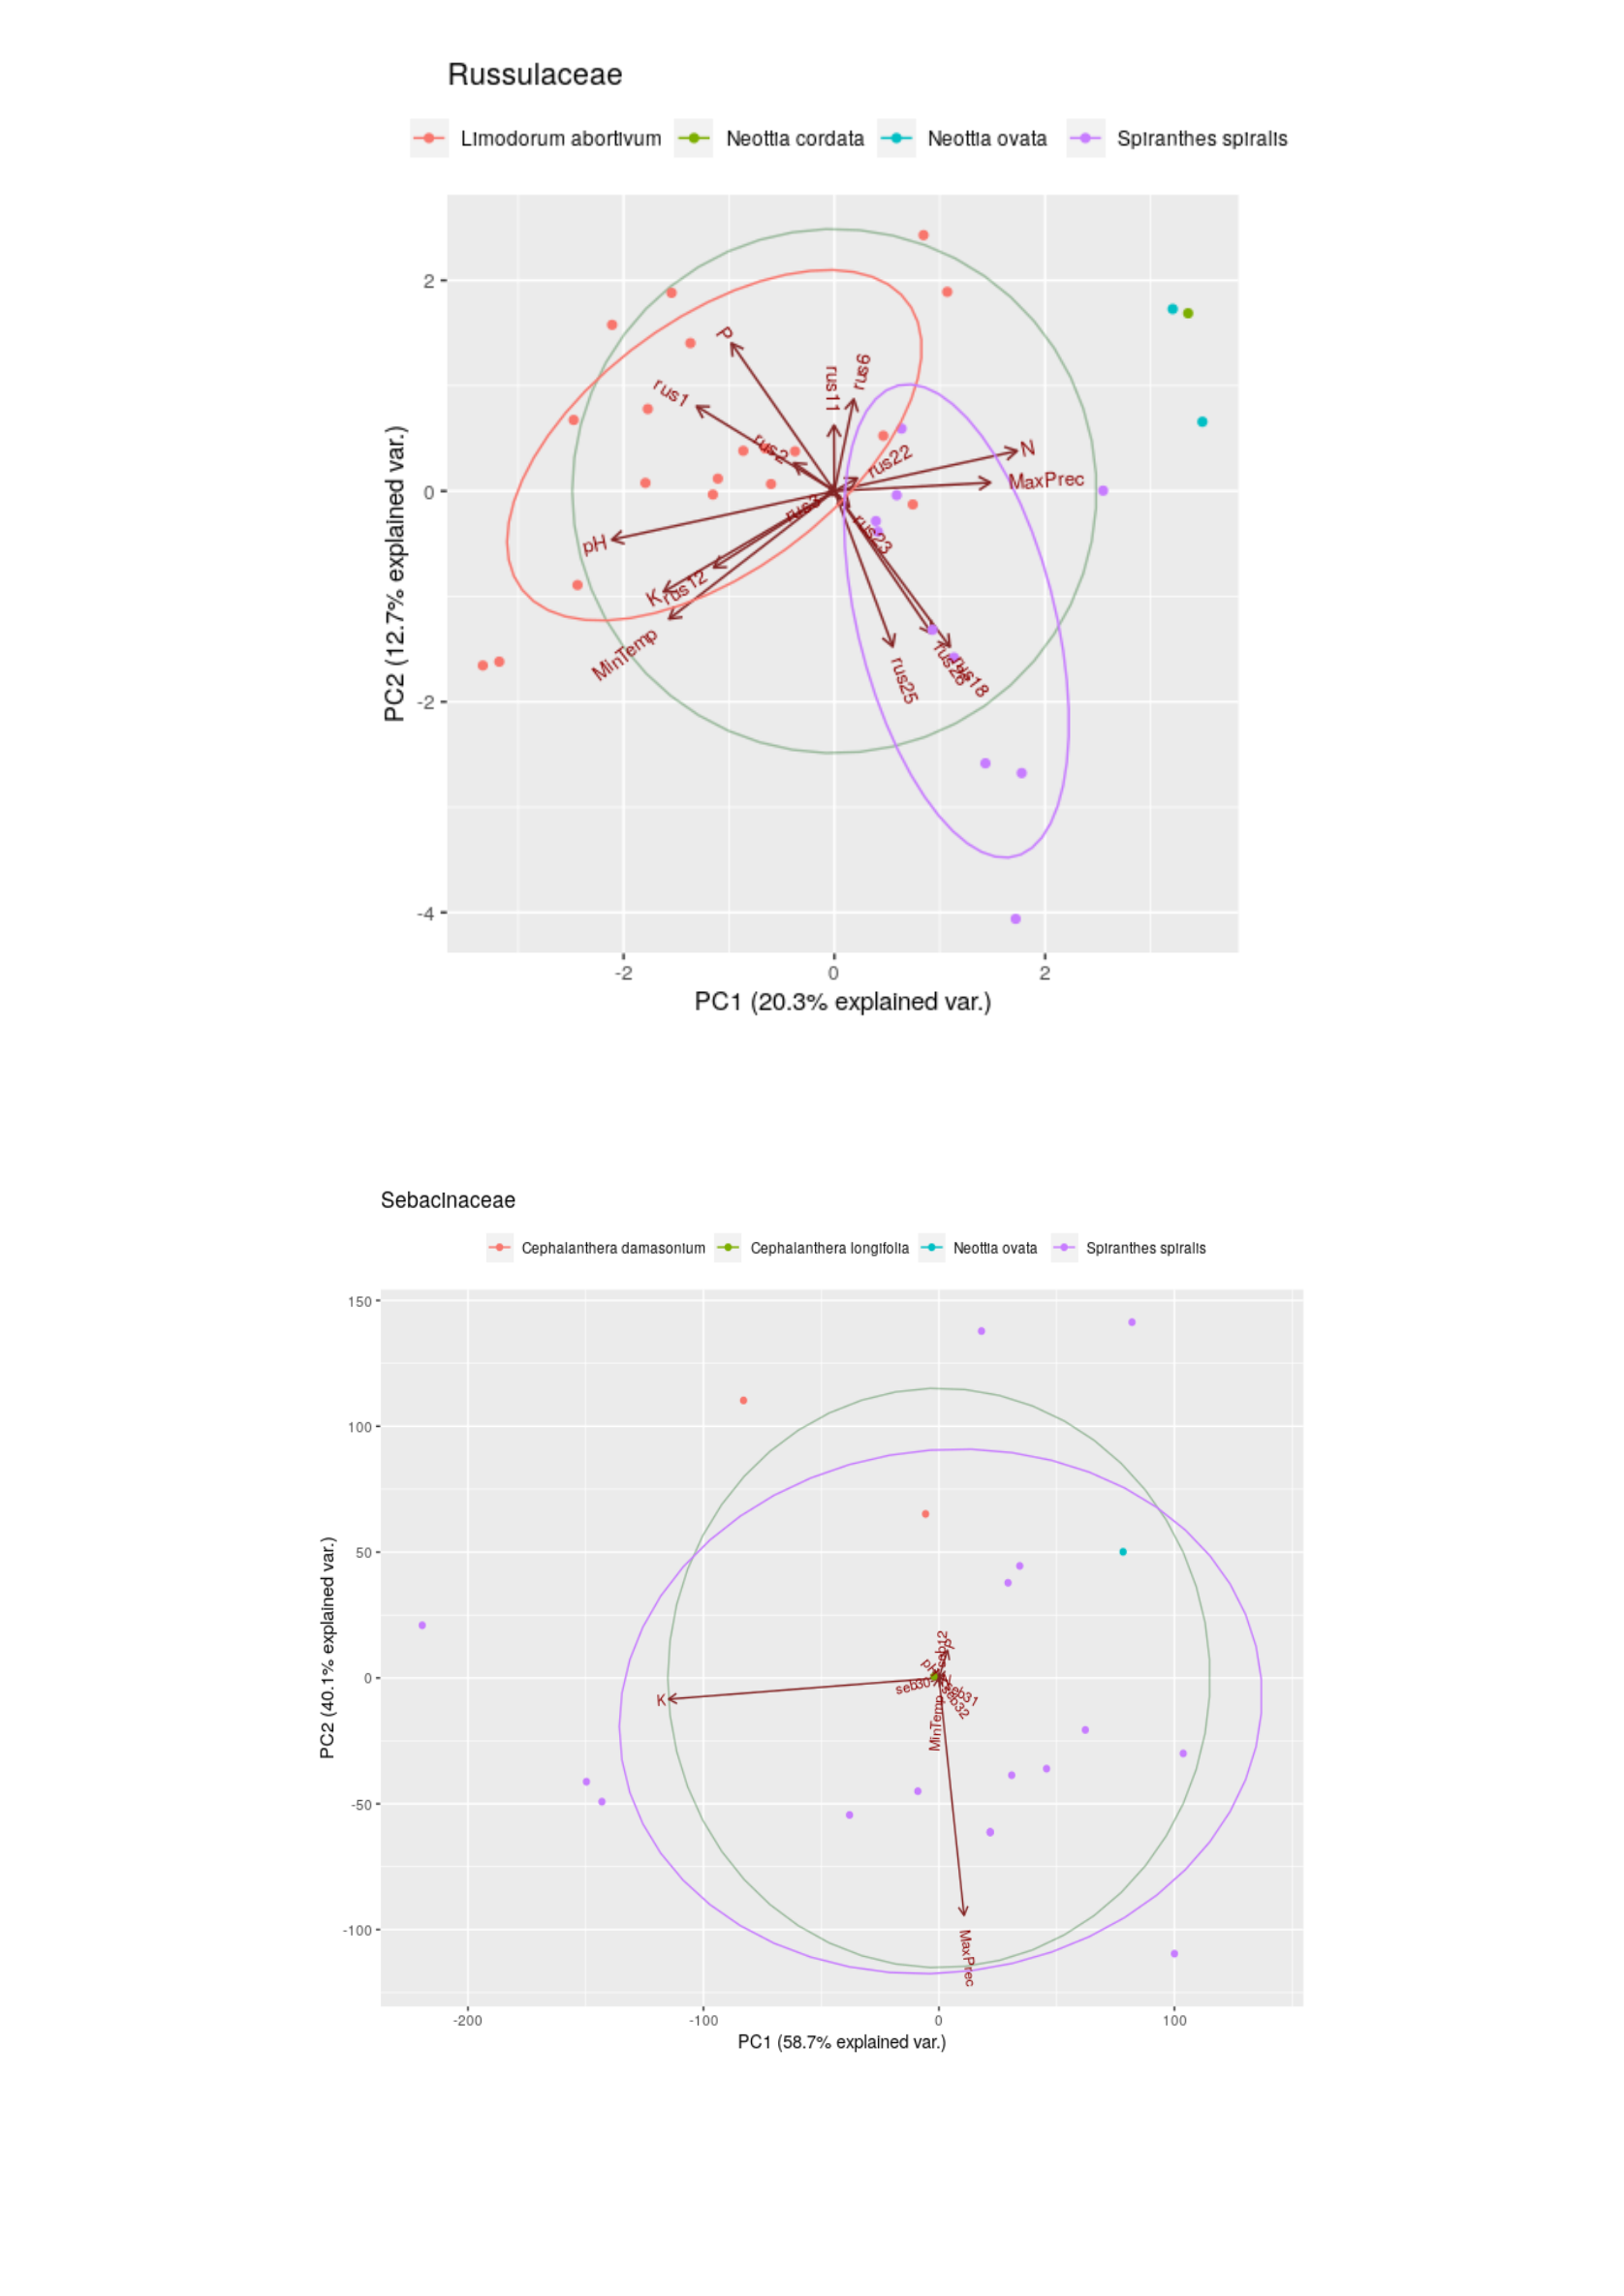
\includegraphics[keepaspectratio,width=\textwidth,height=0.75\textheight]{images/PCArusseb.png}
\caption{PCA of Russulaceae and Sebacinaceae}
\end{figure}

\begin{figure}[htbp]
\centering
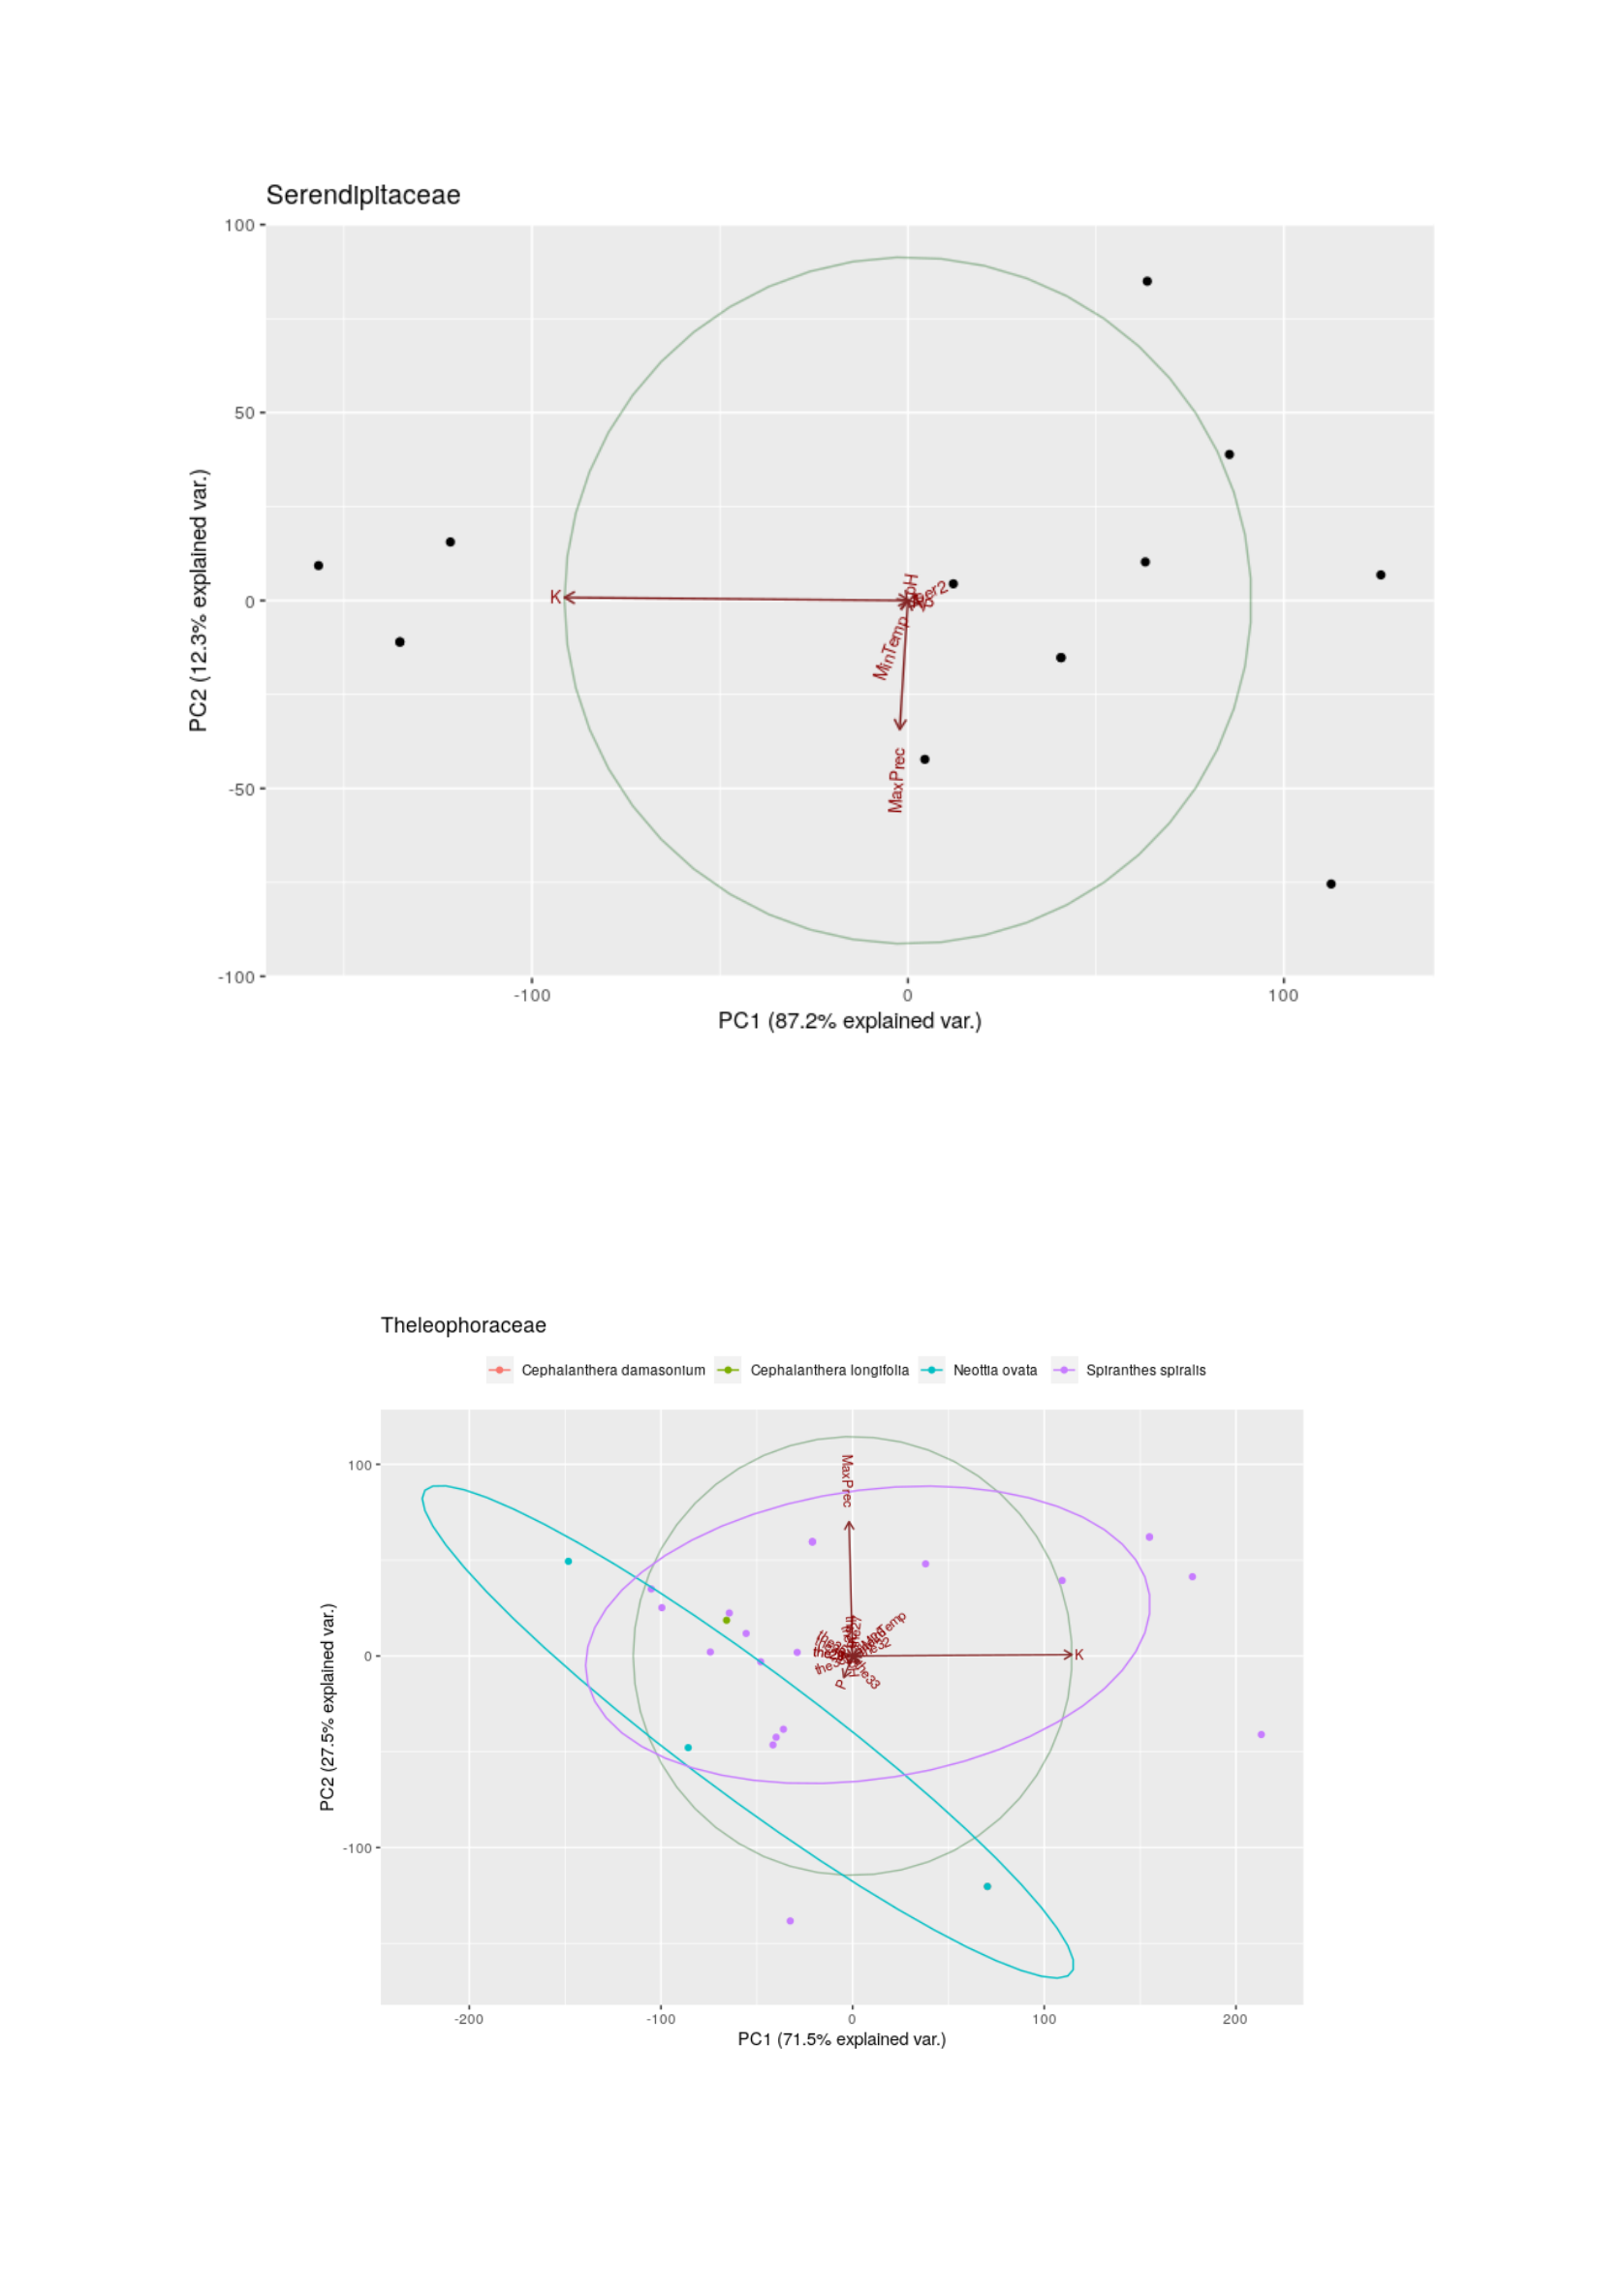
\includegraphics[keepaspectratio,width=\textwidth,height=0.75\textheight]{images/PCAserthe.png}
\caption{PCA of Serendipitaceae and Theleophoraceae}
\end{figure}

\begin{figure}[htbp]
\centering
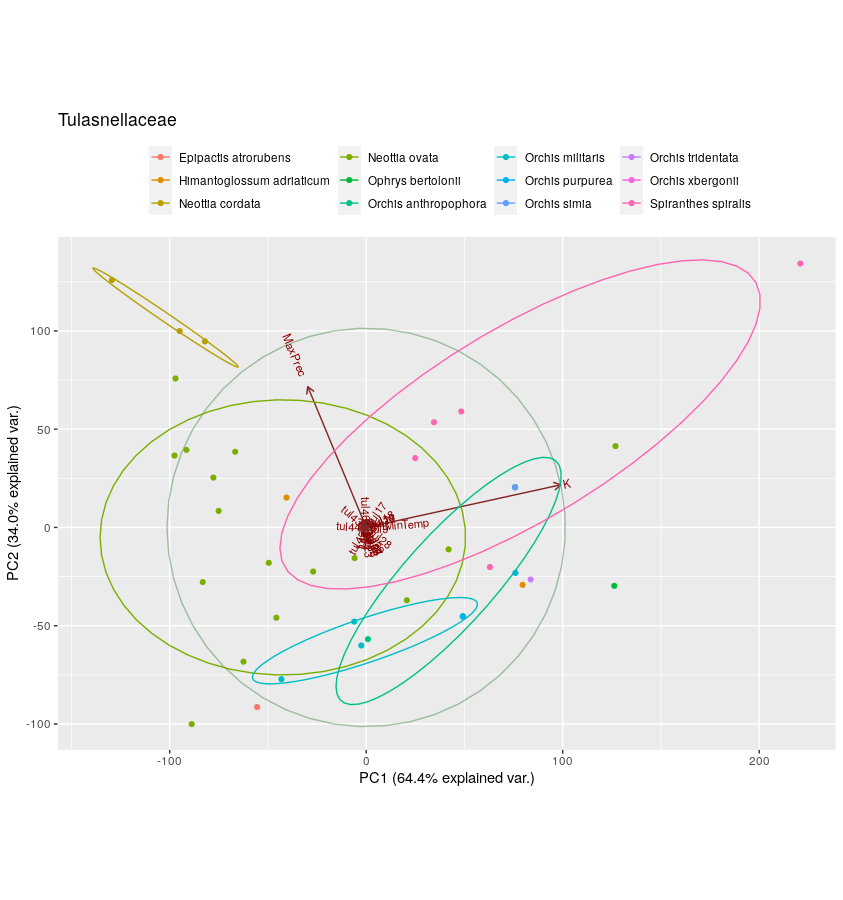
\includegraphics[keepaspectratio,width=\textwidth,height=0.75\textheight]{images/PCAtul.png}
\caption{PCA of Tulasnellaceae}
\end{figure}

\input{latEnd.txt}

\end{document}
